
\clearpage

\section{Explorando PDB4DNA}
\label{sec:MODIFI}
\begin{figure}[htbp]
    \centering
    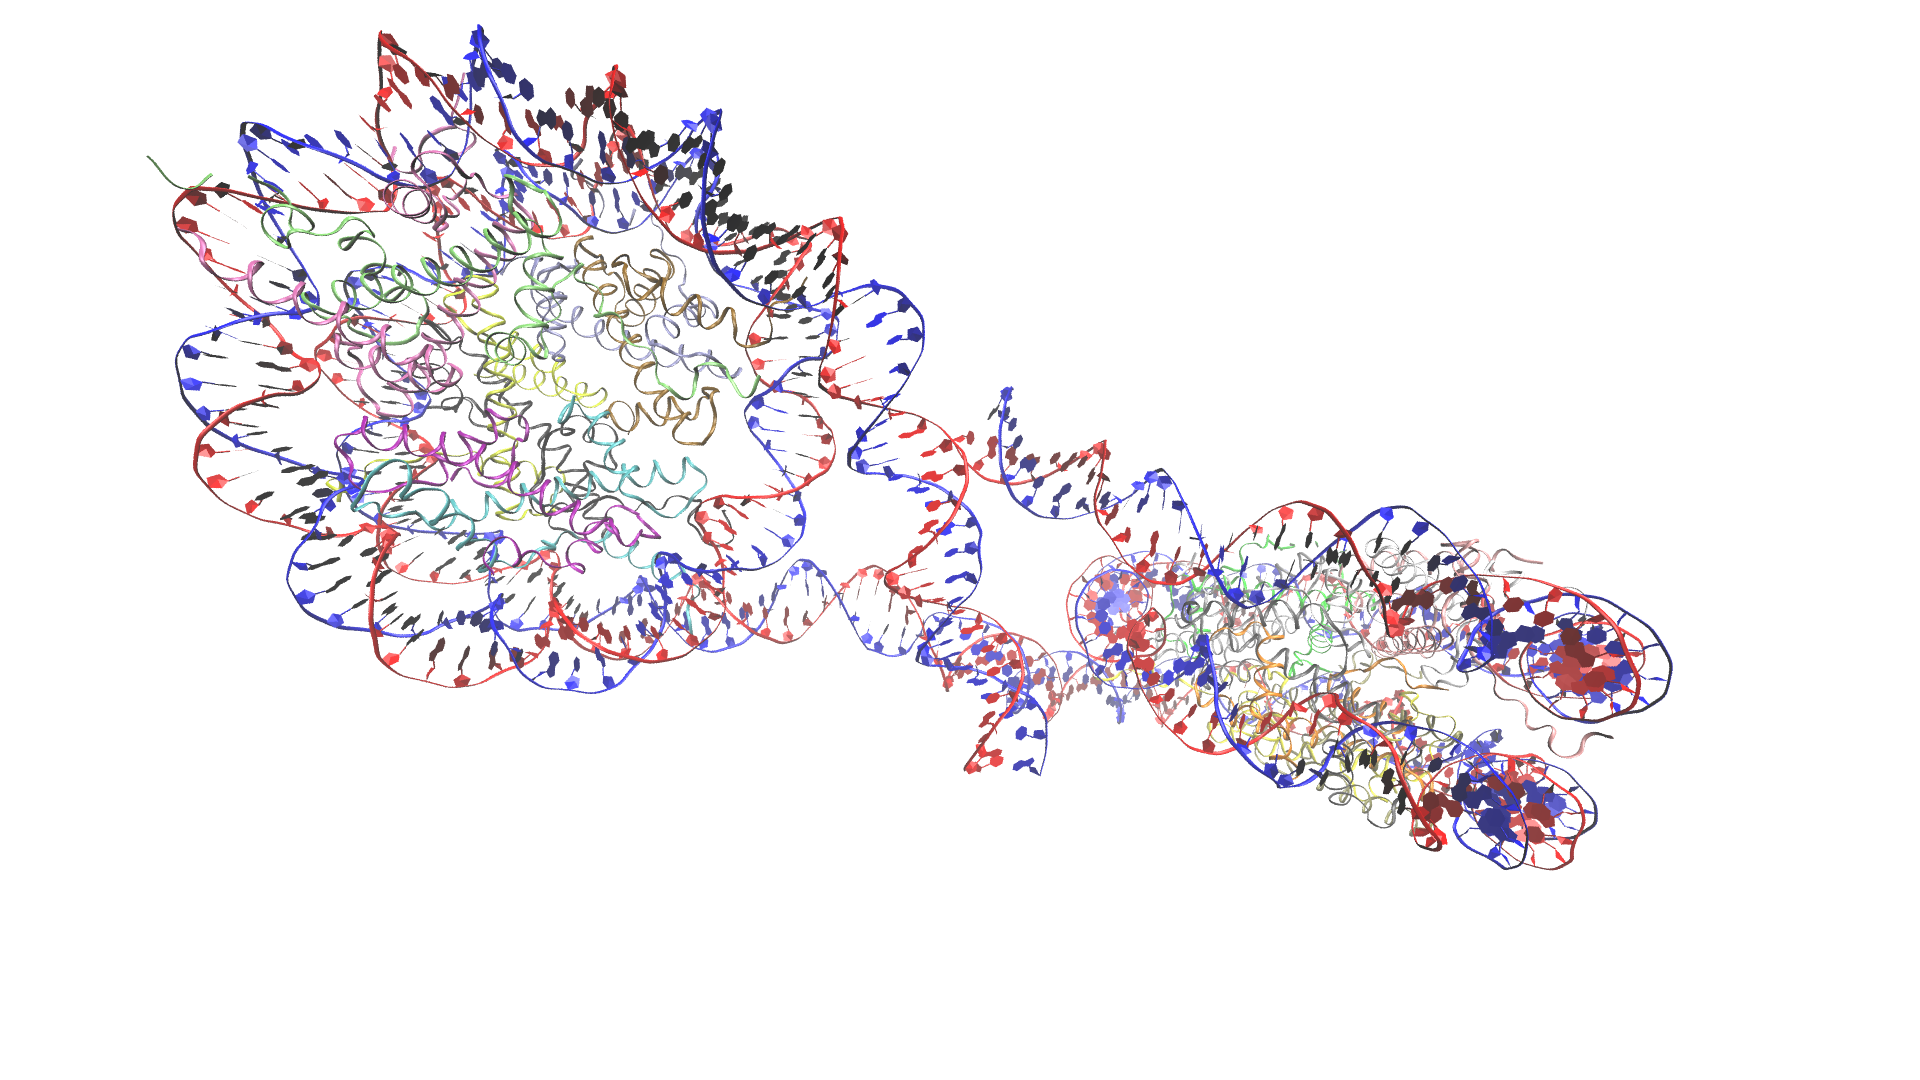
\includegraphics[width=0.8\linewidth]{./Figures/1ZBB.png}
    \caption[Molécula de ADN 1ZBB]{Molécula de ADN 1ZBB vista en VMD}
    \label{fig:1zbb}
\end{figure}

\begin{figure}[htbp]
    \centering
    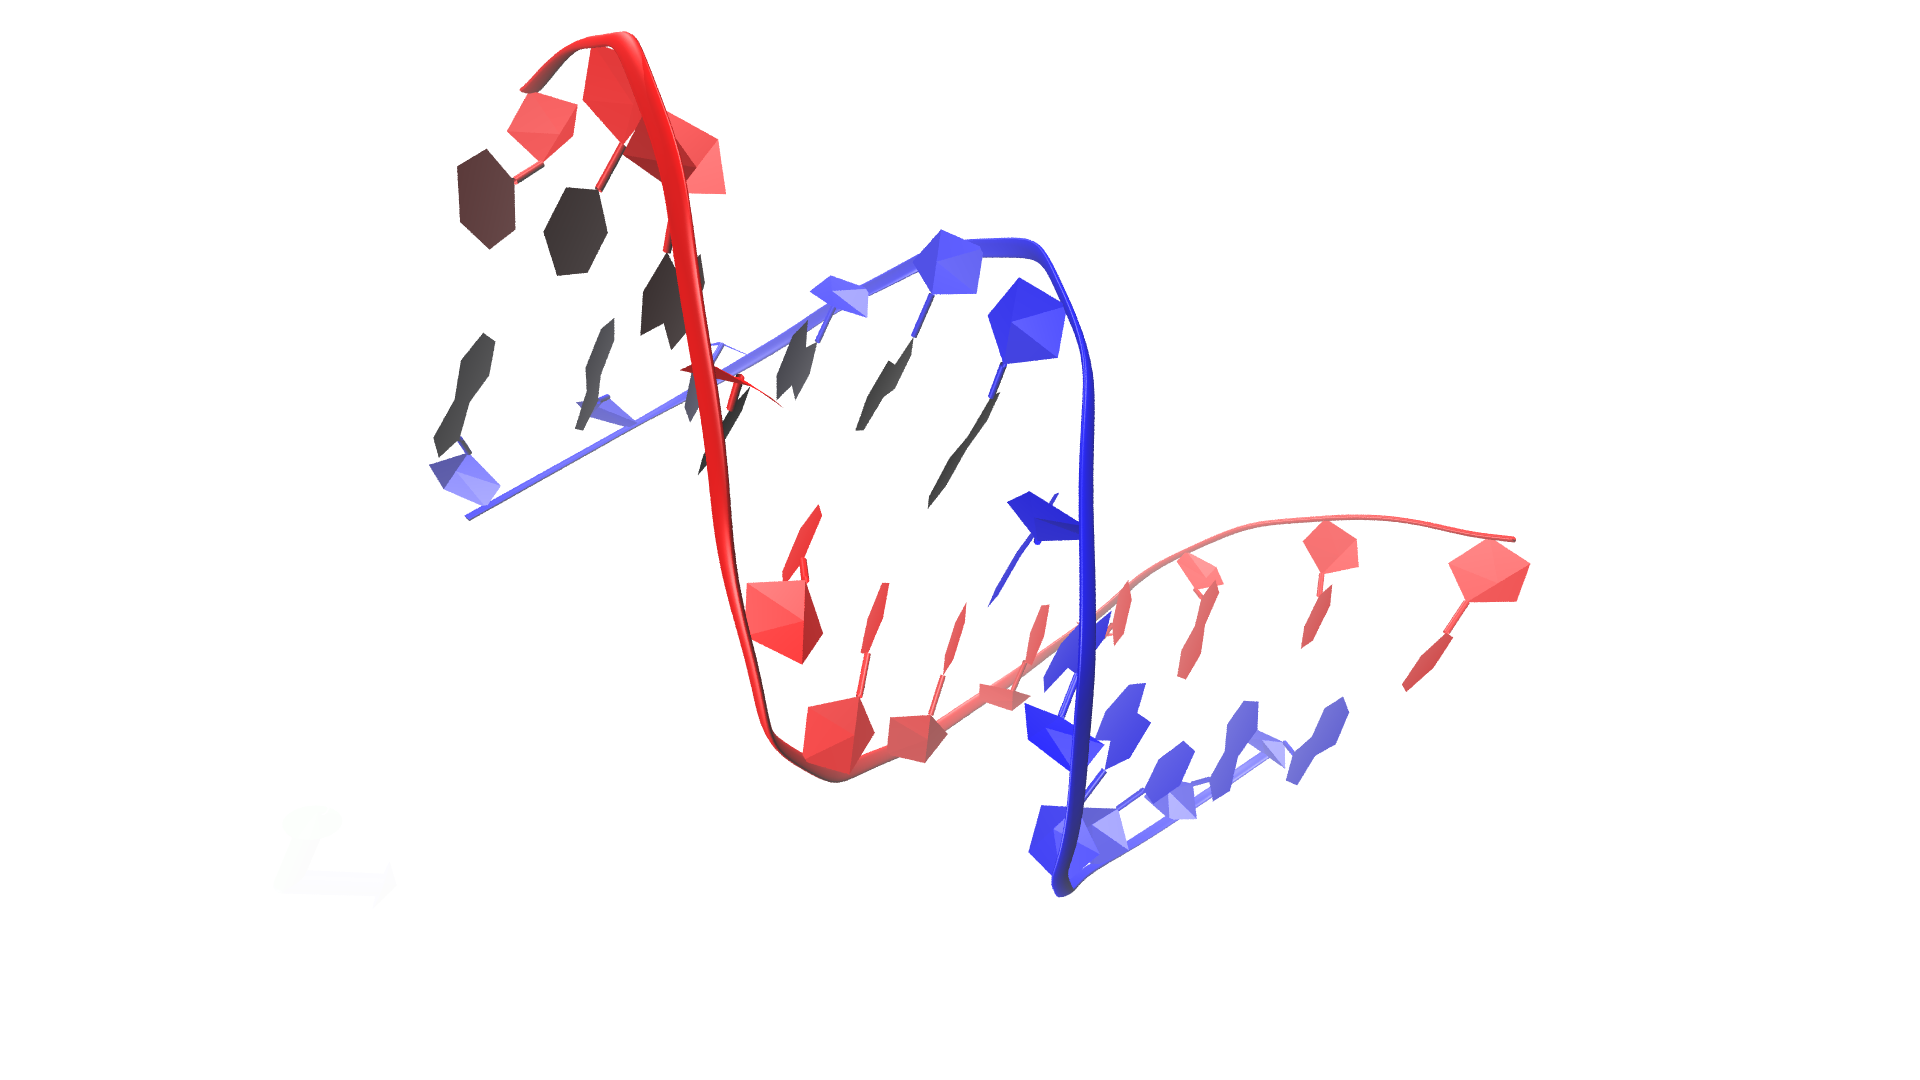
\includegraphics[width=0.8\linewidth]{./Figures/1FZX.png}
    \caption[Molécula de ADN 1FZX]{Molécula de ADN 1FZX vista en VMD}
    \label{fig:1fzx}
\end{figure}
Con tal de entender el código de pdb4dna, sus alcances, y resultados, se hace necesario el explorarlo. Se generaron histogramas de deposición de energía junto con los rompimientos simples y dobles para dos diferentes moléculas de ADN, 1ZBB(véase figura ~\ref{fig:1zbb} ) y 1FZX(véase figura ~\ref{fig:1fzx}), estos se realizaron con 10000 eventos con diferentes valores de energía para un electrón y un baryon con nombres en Geant4 e- y proton respectivamente, véase figuras ~\ref{fig:e}, ~\ref{fig:p}, ~\ref{fig:e2}, ~\ref{fig:p2}, de estos histogramas es interesante notar como los rompimientos simples y doble aumentan hasta cierto valor y luego empiezan a reducirse, esto puede deberse a diversos factores como el tamaño de la molécula y en cuantos enlaces se puede depositar la energía, también es necesario mencionar que en el stepping action la energía y las posiciones donde se deposita la energía se obtiene mediante la librería step y para ser precisos con la siguiente linea de código:
\lstset {language=C++}
\begin{lstlisting}
// Get position and edep of current step
    //
    G4double x = theStep->GetPreStepPoint()->GetPosition().x()/nanometer;
    G4double y = theStep->GetPreStepPoint()->GetPosition().y()/nanometer;
    G4double z = theStep->GetPreStepPoint()->GetPosition().z()/nanometer;
G4double edepStep = theStep->GetTotalEnergyDeposit()/eV;
\end{lstlisting}

Al graficar los baricentros contra estas deposiciones de la energía debido a la partícula(figura ~\ref{fig:edep}) se puede ver en que partes se esta depositando la energía, bien lo que hace el código es filtrar la energía para que el programa genere un histograma de deposición de energía en donde solo se deposito energía en el fosfato o el azúcar, esto lo hace mediante varias lineas de código,primero PDBlic se encarga de leer el pdb y luego de la división de base fosfato y azúcar, mediante el código:

\lstset {language=C++}
\begin{lstlisting}
if(residueListTemp->fResSeq == 1)
            {
              if(iii == 0) BSP = 0; //"Phosphate"
              else if(iii < 8) BSP = 1; //"Sugar"
              else BSP = 2; //"Base"
            }
            else
            {
              if(iii < 4) BSP = 0; //"Phosphate"
              else if(iii < 11) BSP = 1; //"Sugar"
              else BSP = 2; //"Base"
            }
\end{lstlisting}
se encarga de dar un valor numerico al fosfato 0, al azucar 1 y a la base 0, luego en el stepping action si se encuentra un golpe ya sea en el azucar o en el fosfato se retorna ese valor de energía, esto se hace mediante:
\lstset {language=C++}
\begin{lstlisting}
int numStrand=0;
  int numNucl=0;
  int intResidue=-1; // 0 for Phospat, 1 for Sugar, 2 for Base
  unsigned short int hit = (fpDetector->GetPDBlib()).ComputeMatchEdepDNA(
      fpDetector->GetBarycenterList(),
      fpDetector->GetMoleculeList(),
      x*10., y*10., z*10.,// x10 => angstrom<->nm
      numStrand, numNucl, intResidue);

  if (hit==1)
  {
    if ((intResidue==0)||(intResidue==1)) //Edep in Phosphate or Sugar
    {
      fpEventAction->AddEdepToNucleotide(numStrand,numNucl,edepStep);
      return true;
    }
    else
    {
      return false;
    }
    \end{lstlisting}

    Esto serviría en primera instancia, reemplazando los valores, para analizar daño de las bases, pero debido a que no tenemos noción de como se evaluá el daño por radiación en bases no se realizara, por ahora.

    
\begin{figure}
\centering
\begin{subfigure}{.5\textwidth}
  \centering
  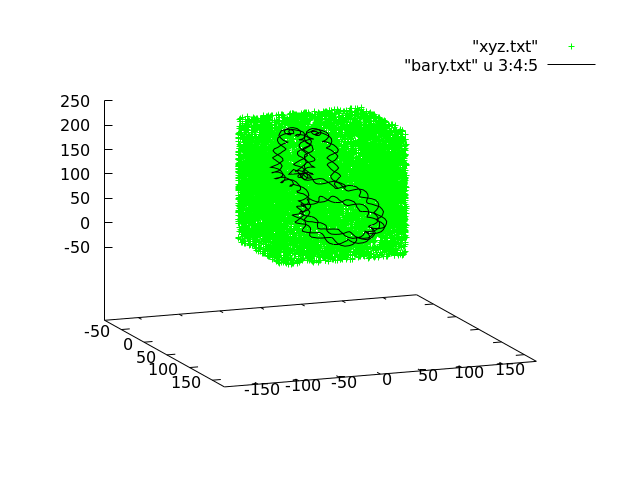
\includegraphics[width=1\linewidth]{./Figures/dep.png}
  \caption{Vista lateral}
  \label{fig:subeio1}
\end{subfigure}%
\begin{subfigure}{.5\textwidth}
  \centering
  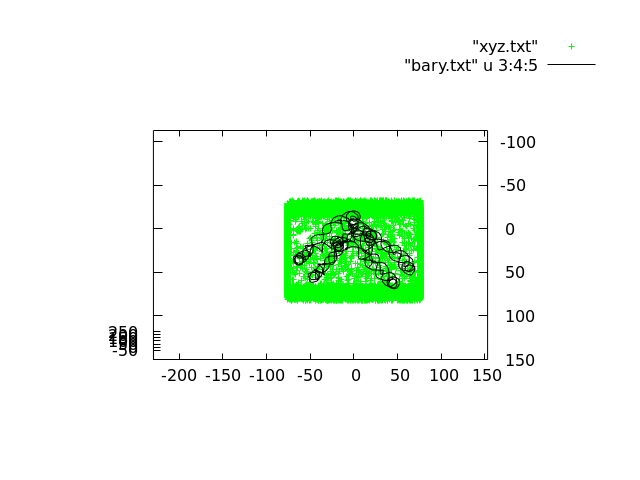
\includegraphics[width=1\linewidth]{./Figures/dep1.png}
  \caption{Vista superior}
  \label{fig:subeio2}
\end{subfigure}
\caption[Puntos de deposición de energía 1ZBB]{Puntos donde la partícula deposita energía en verde, y baricentros de 1ZBB en negro.}
\label{fig:edep}
\end{figure}




\begin{figure}
\centering
\begin{subfigure}{.5\textwidth}
  \centering
  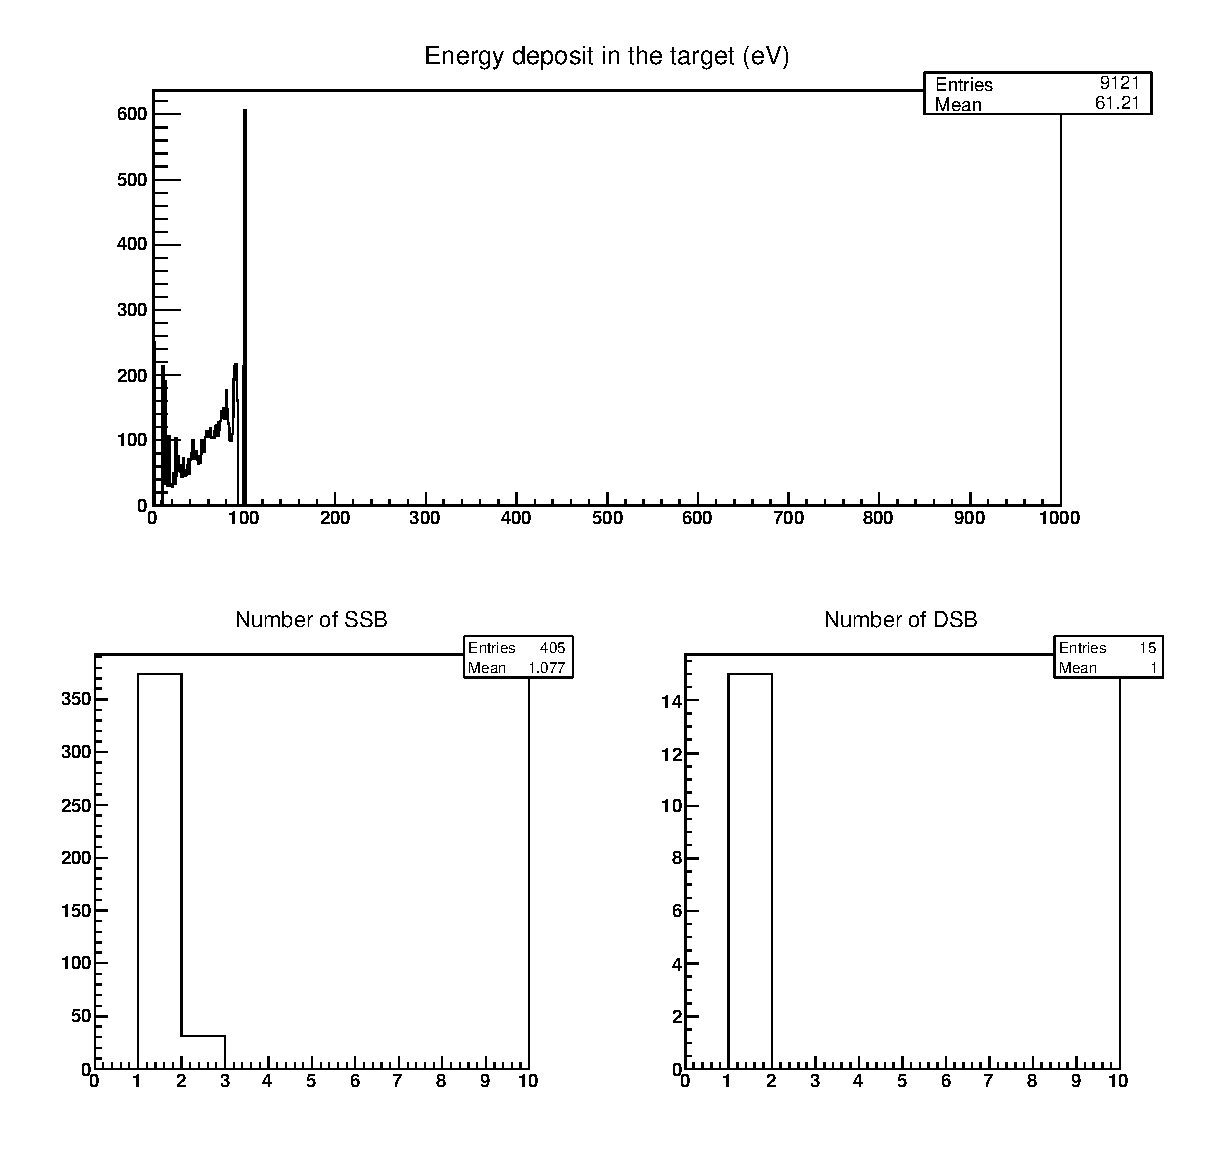
\includegraphics[width=.78\linewidth]{./Figures/e-100ev.eps}
  \caption{100 eV}
  \label{fig:subei1}
\end{subfigure}%
\begin{subfigure}{.5\textwidth}
  \centering
  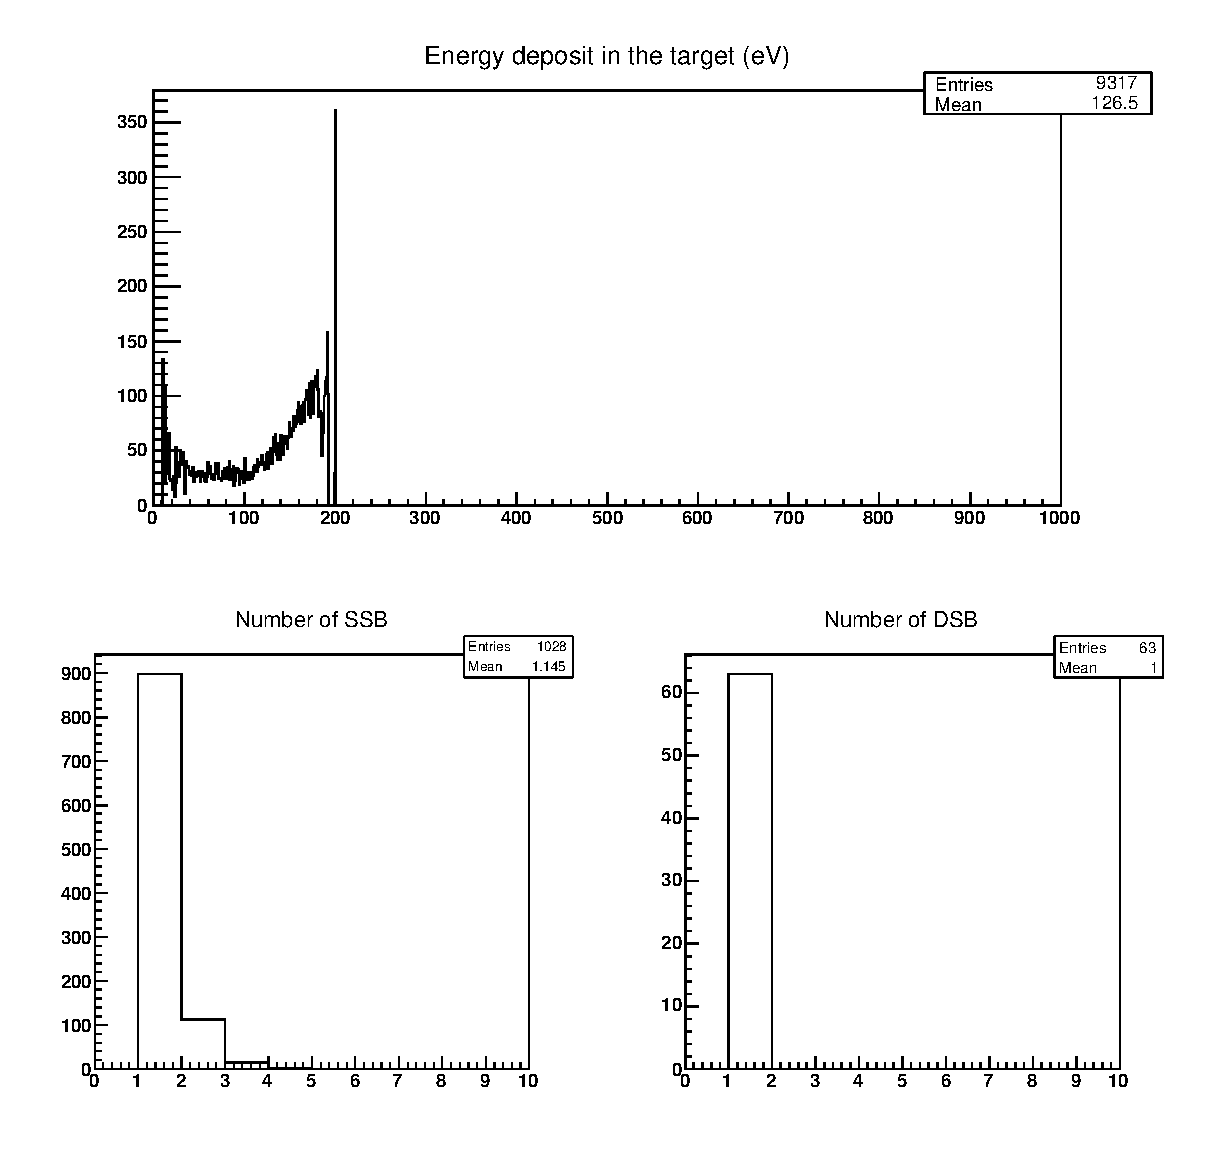
\includegraphics[width=.78\linewidth]{./Figures/e-200ev.eps}
  \caption{200 eV}
  \label{fig:subei2}
\end{subfigure}
\begin{subfigure}{.5\textwidth}
  \centering
  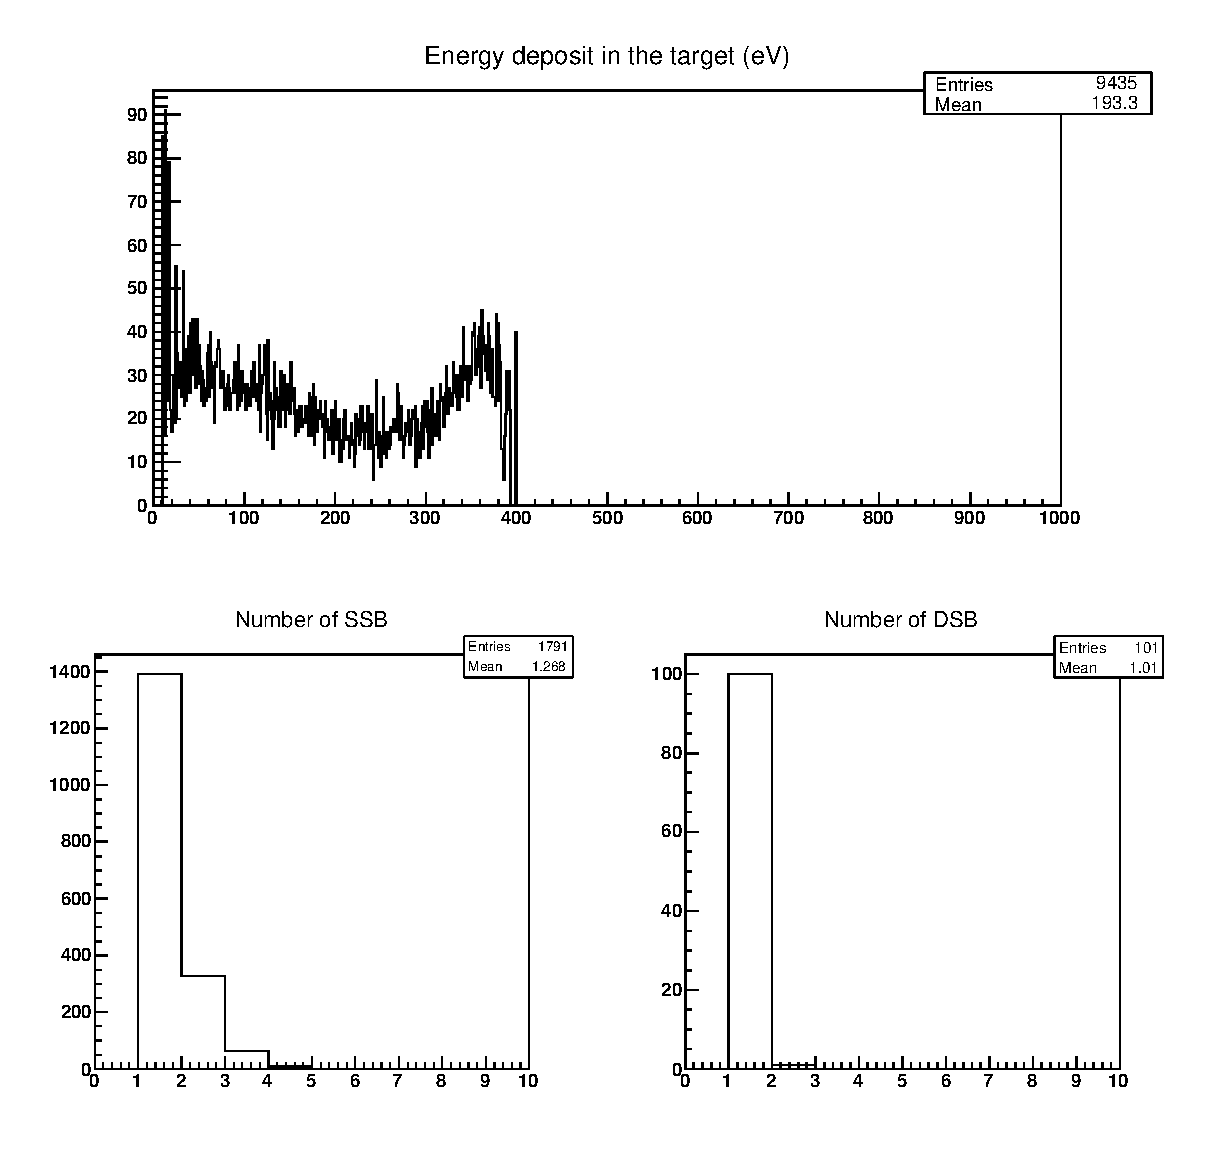
\includegraphics[width=.78\linewidth]{./Figures/e-400ev.eps}
  \caption{400 eV}
  \label{fig:subei3}
\end{subfigure}%
\begin{subfigure}{.5\textwidth}
  \centering
  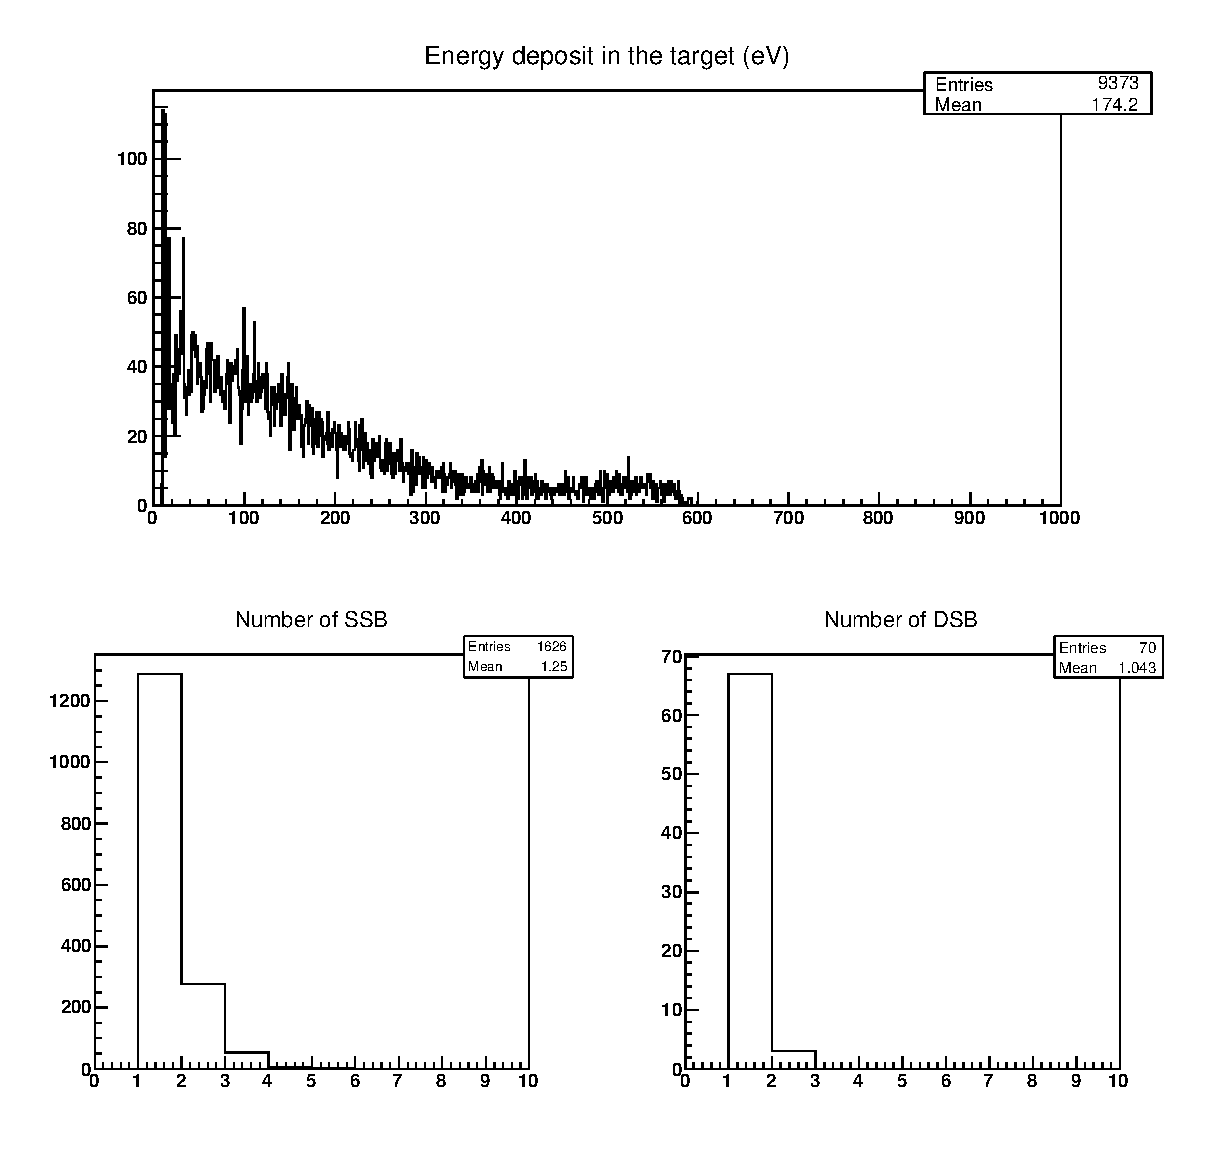
\includegraphics[width=.78\linewidth]{./Figures/e-600.eps}
  \caption{600 eV}
  \label{fig:subei4}
\end{subfigure}
\begin{subfigure}{.5\textwidth}
  \centering
  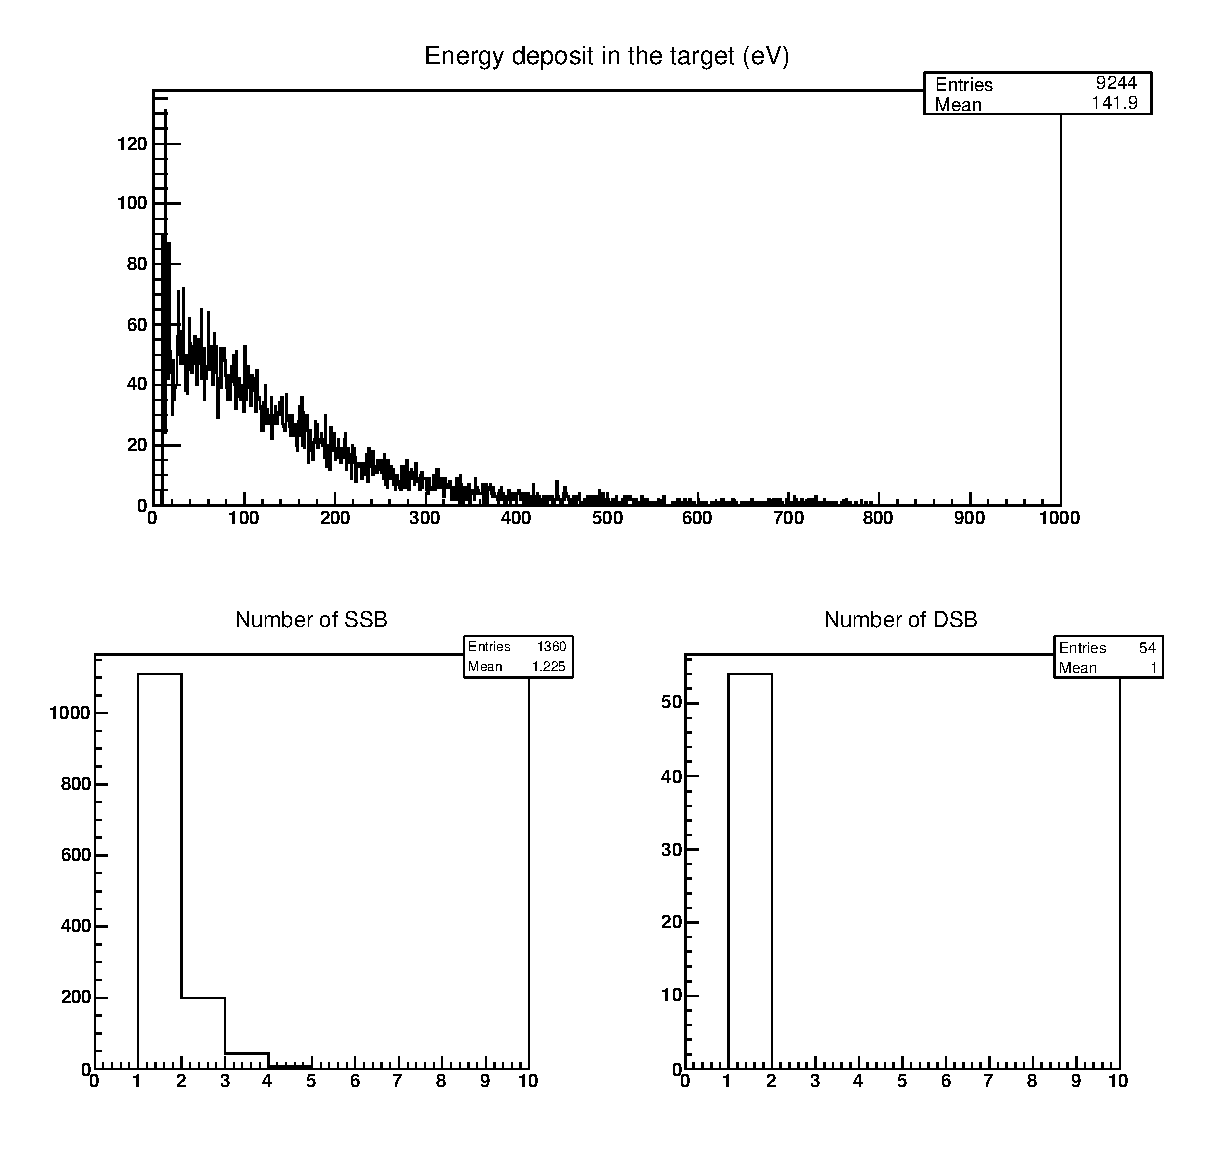
\includegraphics[width=.78\linewidth]{./Figures/e-800ev.eps}
  \caption{800 eV}
  \label{fig:subei5}
\end{subfigure}%
\begin{subfigure}{.5\textwidth}
  \centering
  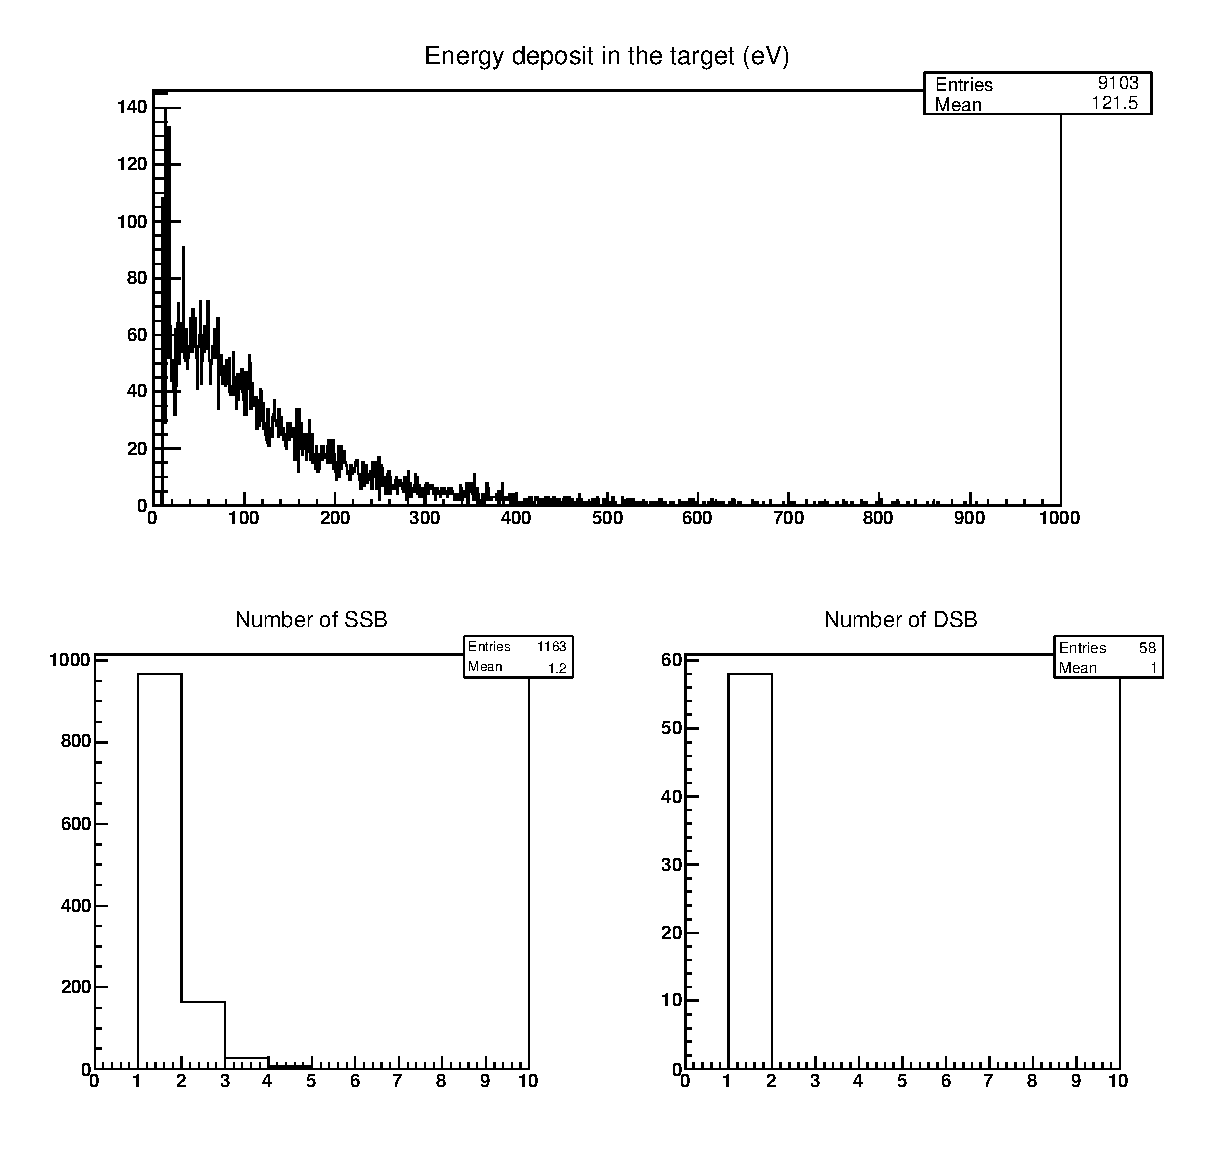
\includegraphics[width=.78\linewidth]{./Figures/e1kev.eps}
  \caption{1 keV}
  \label{fig:subei6}
\end{subfigure}
\begin{subfigure}{.5\textwidth}
  \centering
  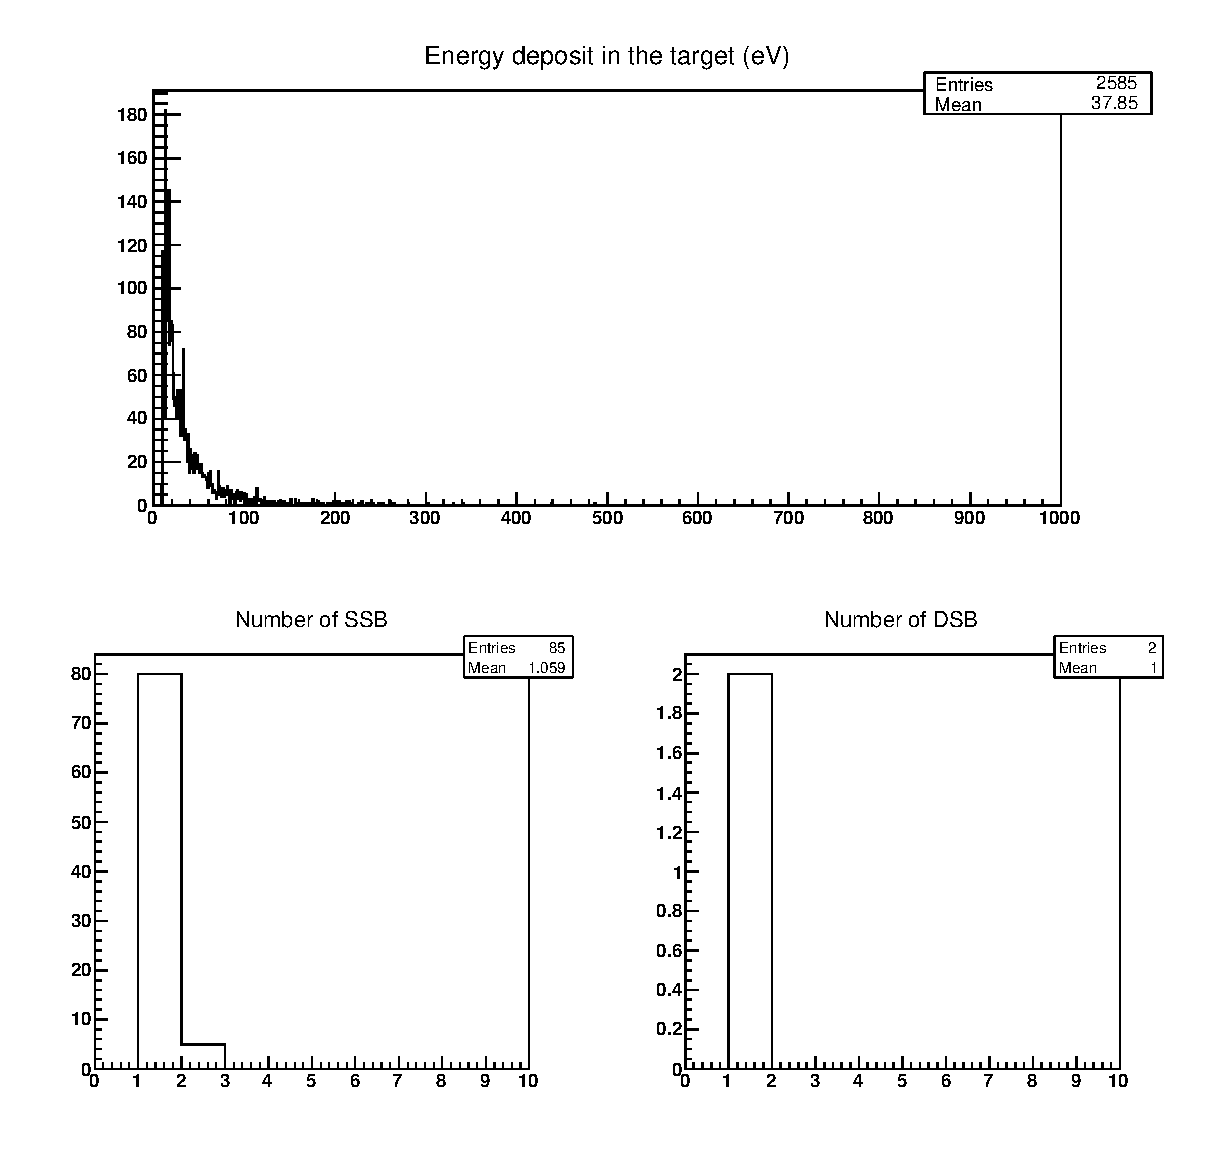
\includegraphics[width=.78\linewidth]{./Figures/e20kev.eps}
  \caption{20 keV}
  \label{fig:subei7}
\end{subfigure}%
\begin{subfigure}{.5\textwidth}
  \centering
  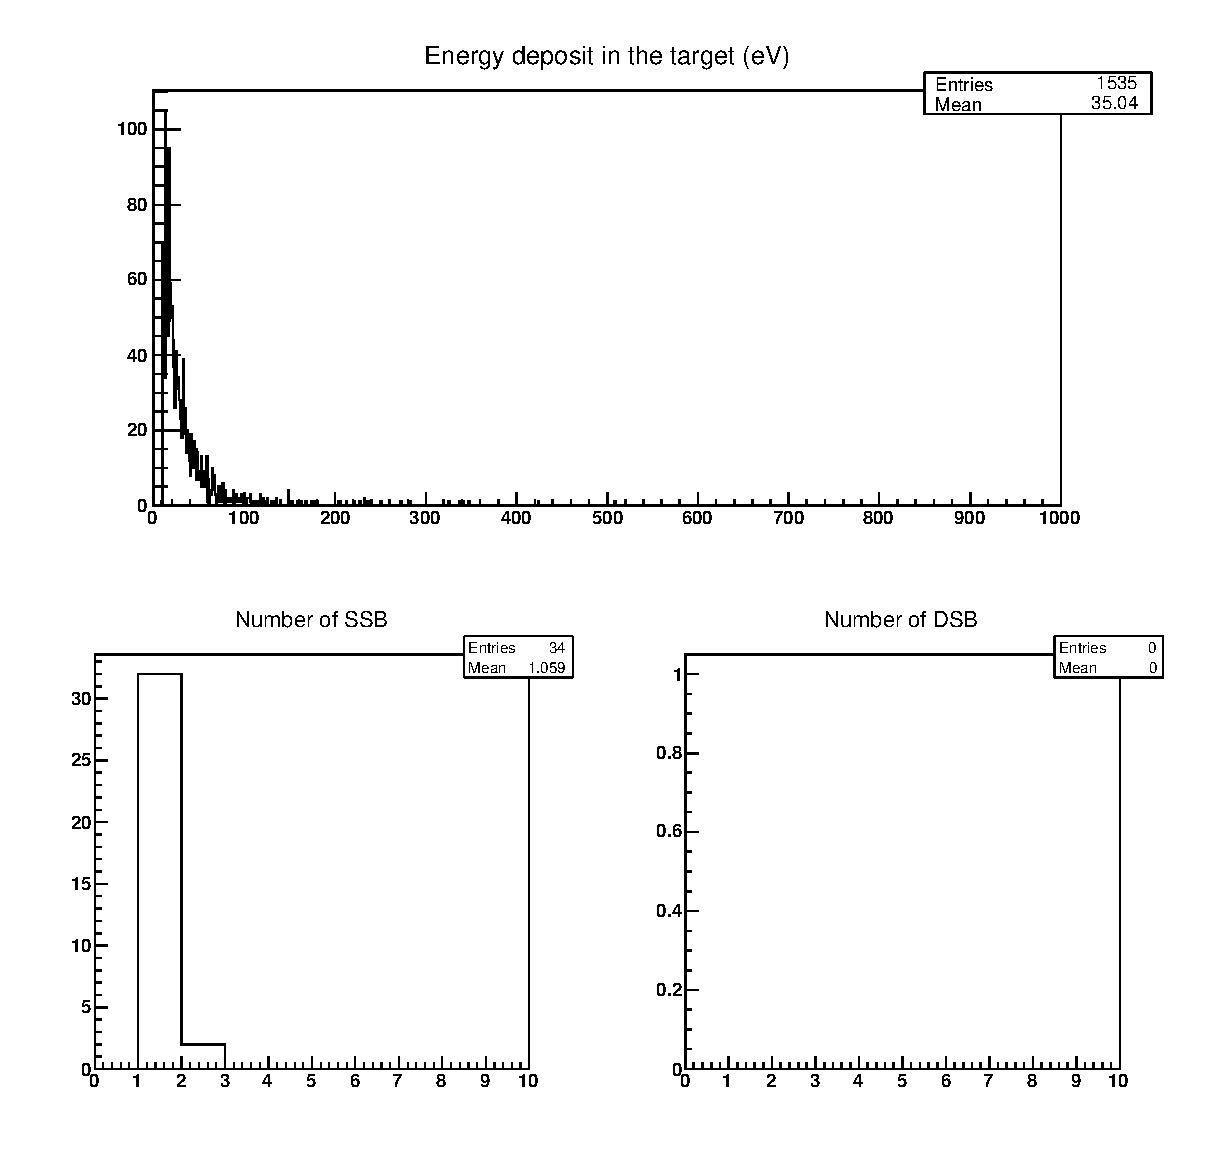
\includegraphics[width=.78\linewidth]{./Figures/e40kev.eps}
  \caption{40 keV}
  \label{fig:subei8}
\end{subfigure}
\caption{Rompimientos simples y dobles para 1ZBB ($e-$)}
\label{fig:e}
\end{figure}

\begin{figure}
\centering
\begin{subfigure}{.5\textwidth}
  \centering
  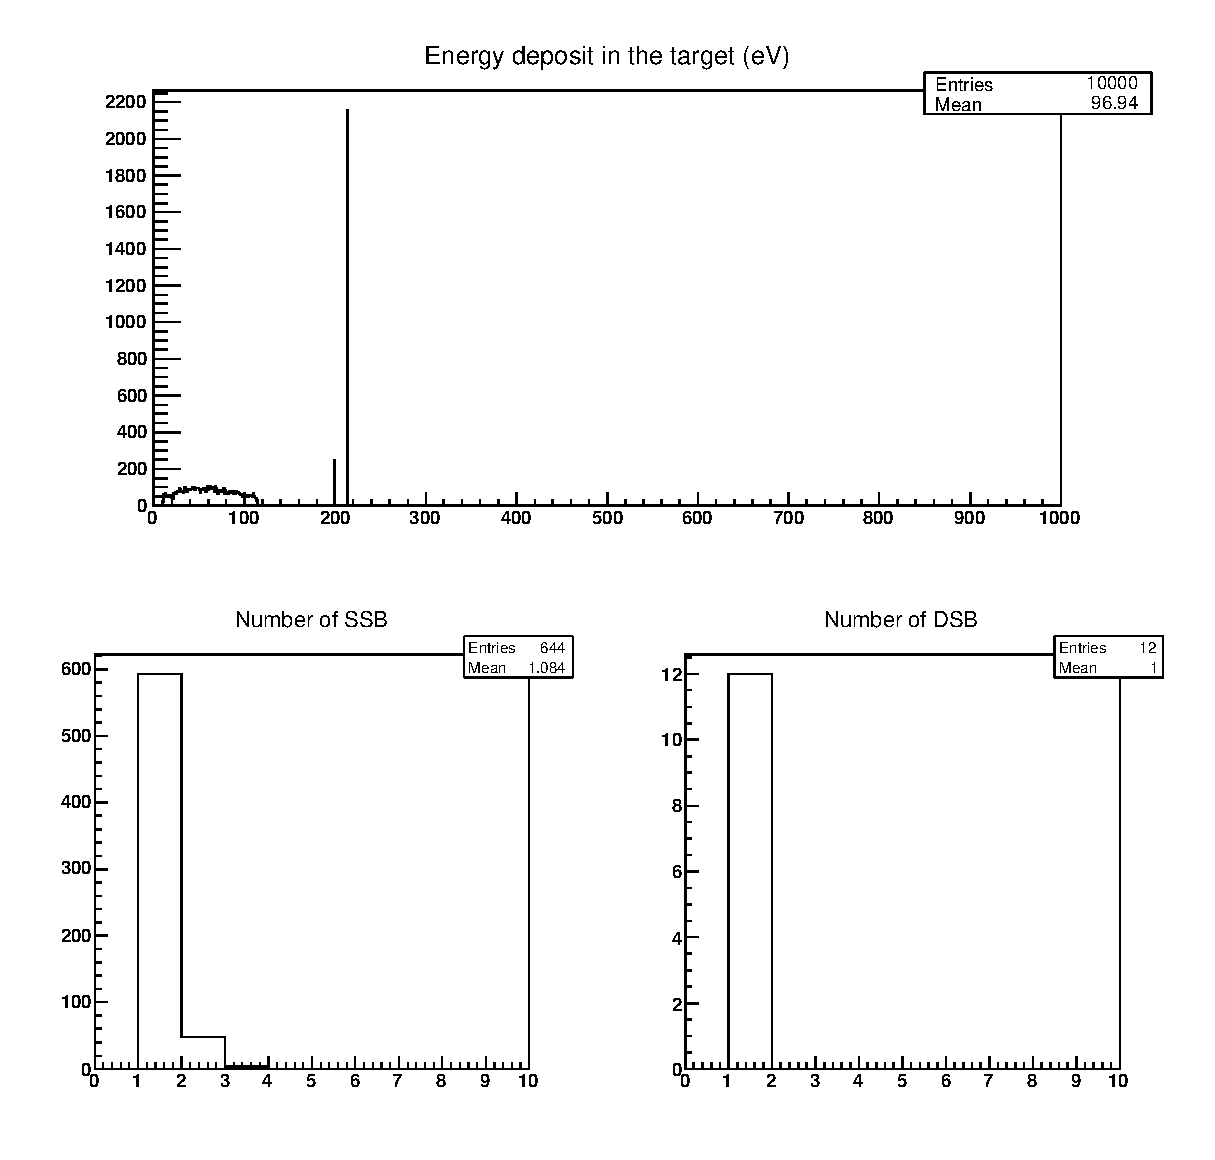
\includegraphics[width=.78\linewidth]{./Figures/proton200eV.eps}
  \caption{200 eV}
  \label{fig:sub1}
\end{subfigure}%
\begin{subfigure}{.5\textwidth}
  \centering
  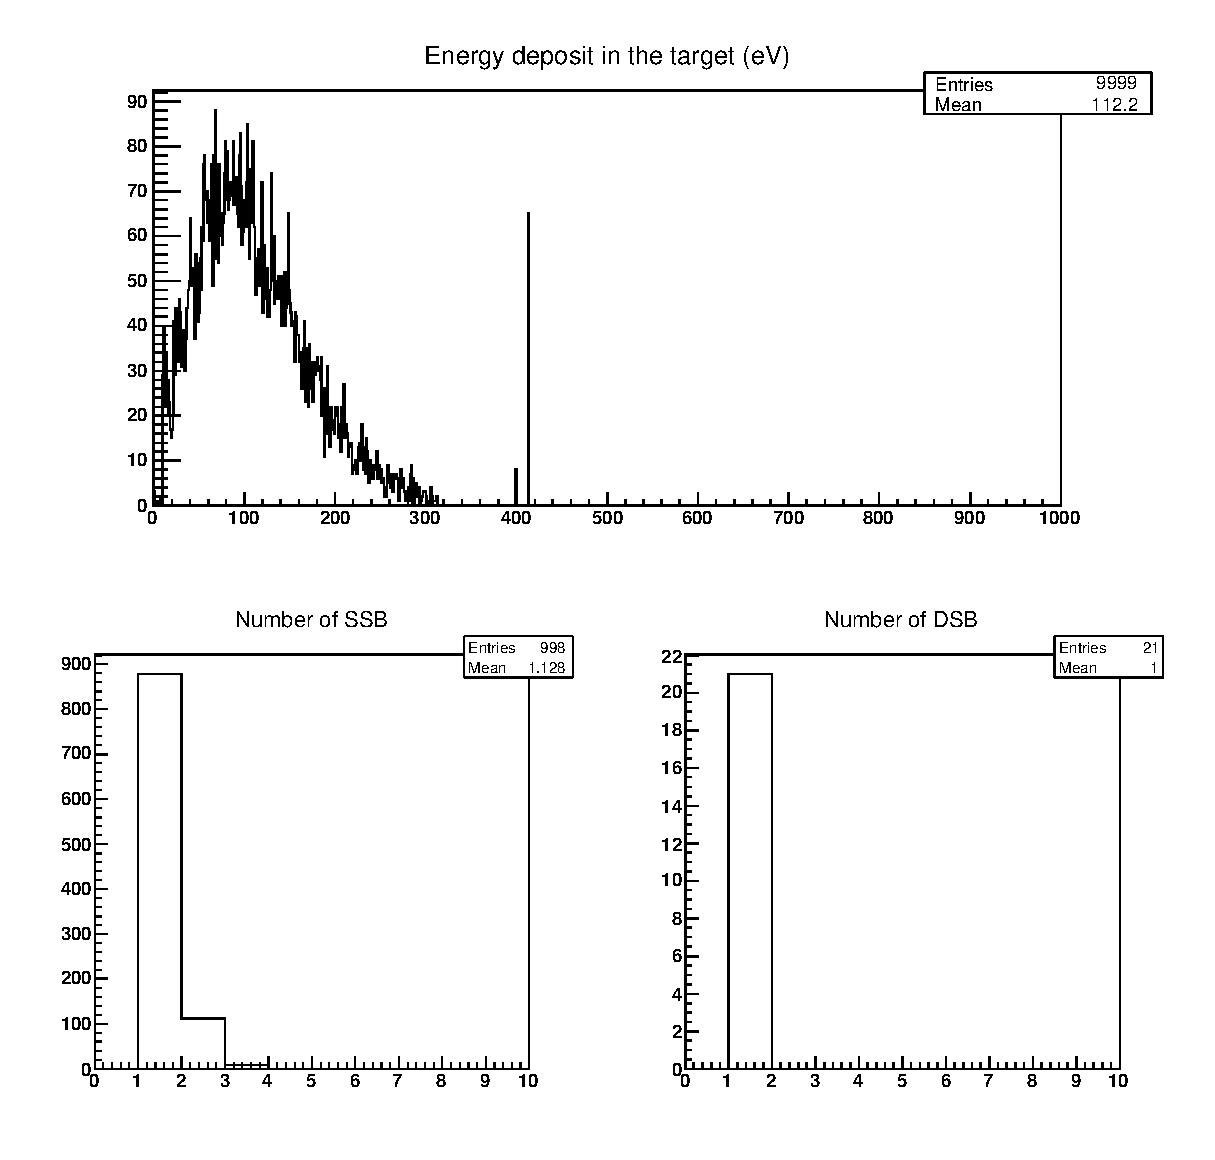
\includegraphics[width=.78\linewidth]{./Figures/proton400eV.eps}
  \caption{400 eV}
  \label{fig:sub2}
\end{subfigure}
\begin{subfigure}{.5\textwidth}
  \centering
  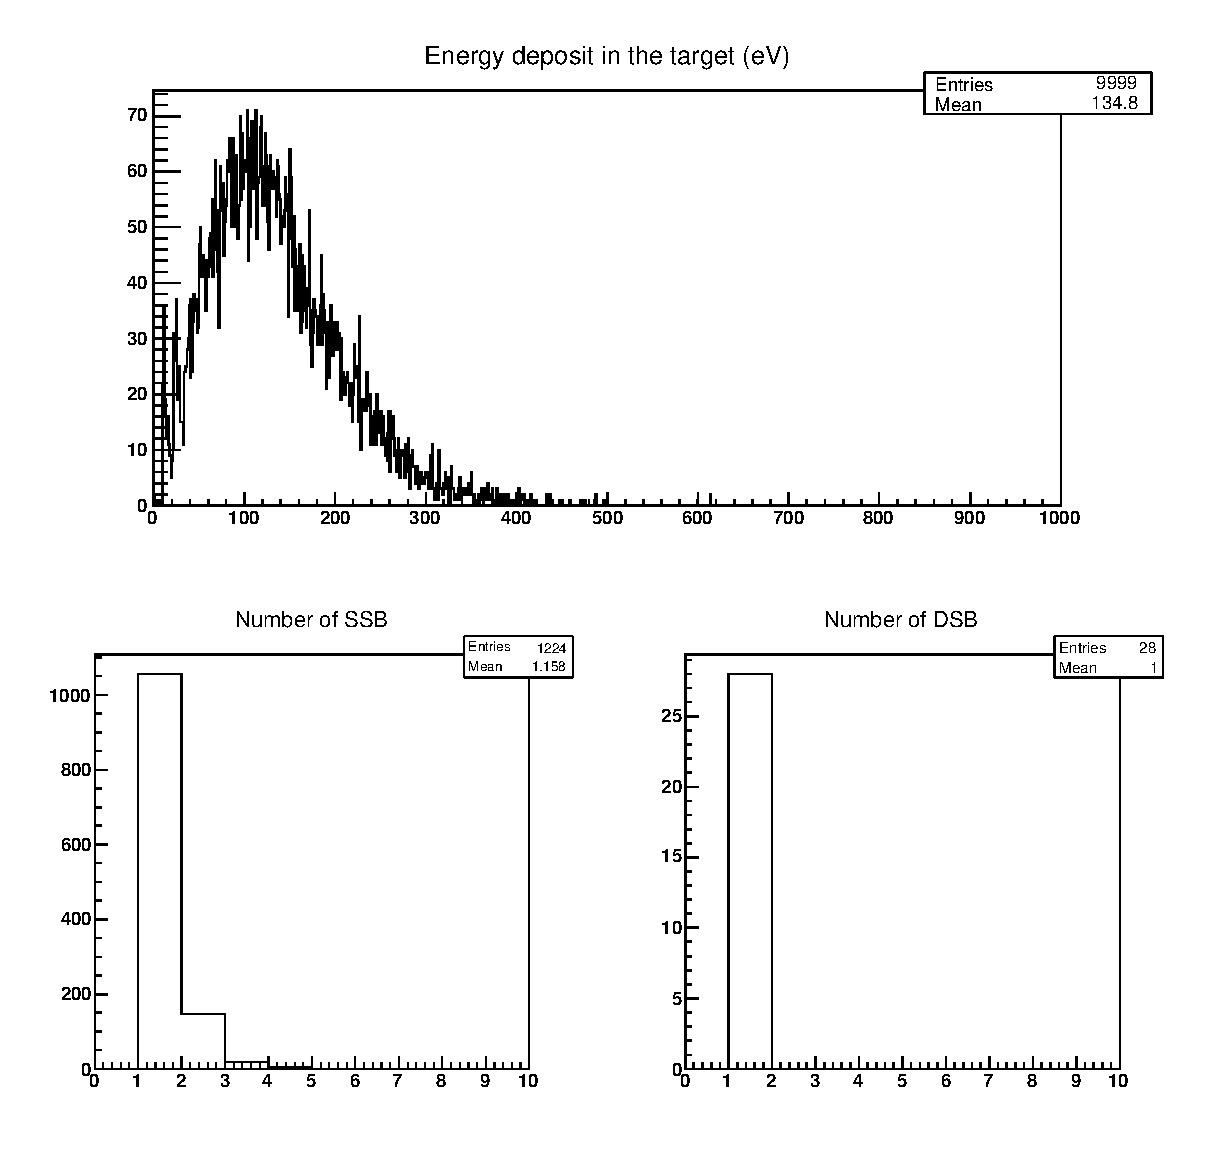
\includegraphics[width=.78\linewidth]{./Figures/proton600eV.eps}
  \caption{600 eV}
  \label{fig:sub3}
\end{subfigure}%
\begin{subfigure}{.5\textwidth}
  \centering
  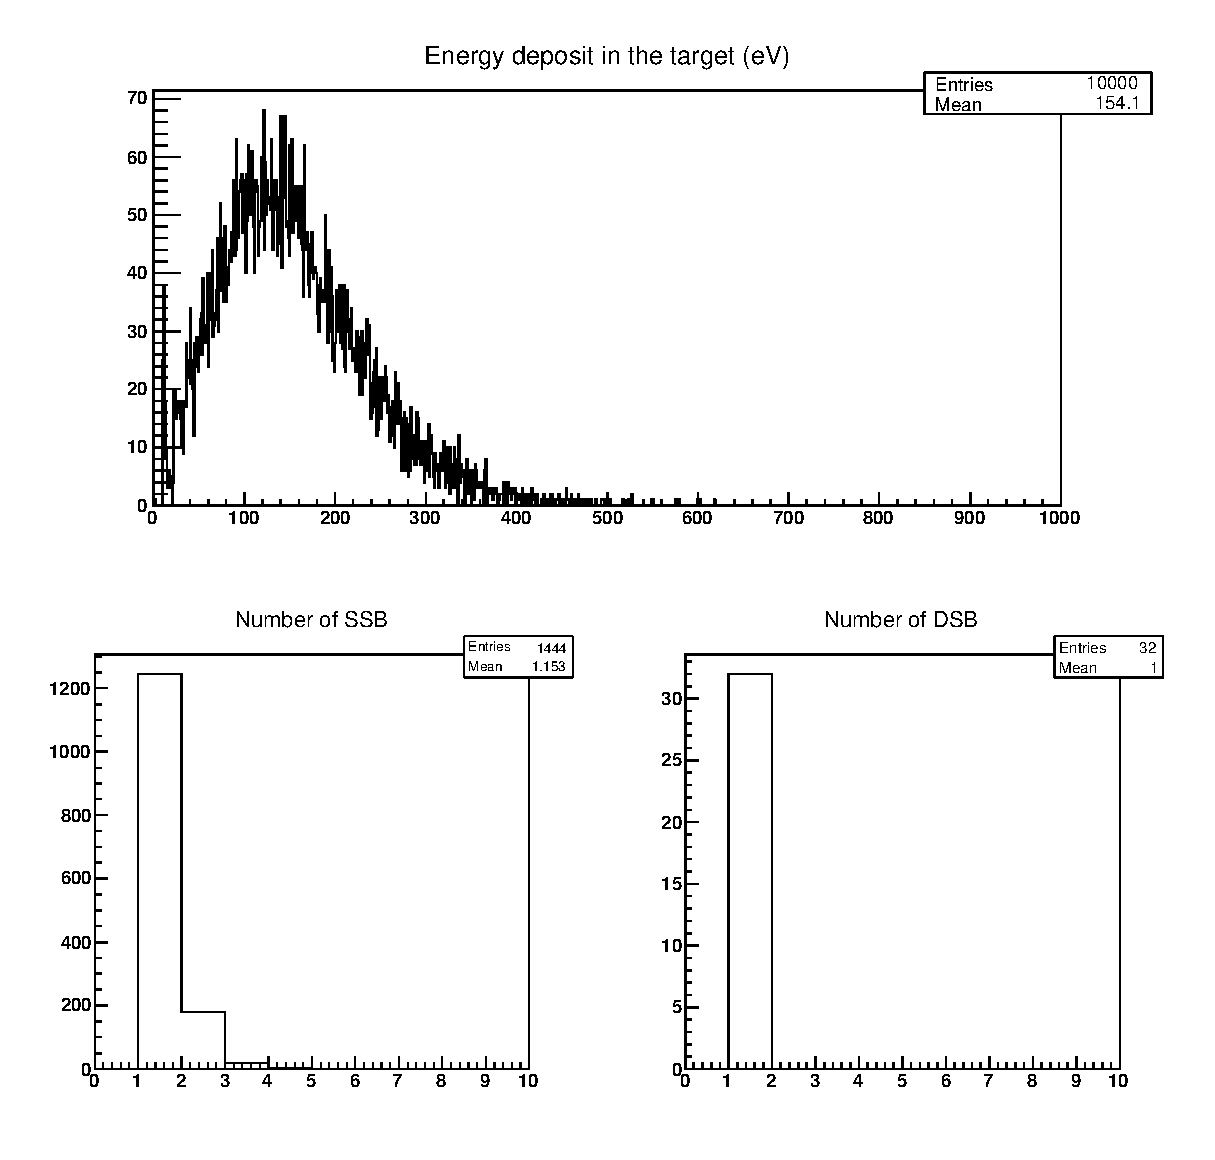
\includegraphics[width=.78\linewidth]{./Figures/proton800eV.eps}
  \caption{800 eV}
  \label{fig:sub4}
\end{subfigure}
\begin{subfigure}{.5\textwidth}
  \centering
  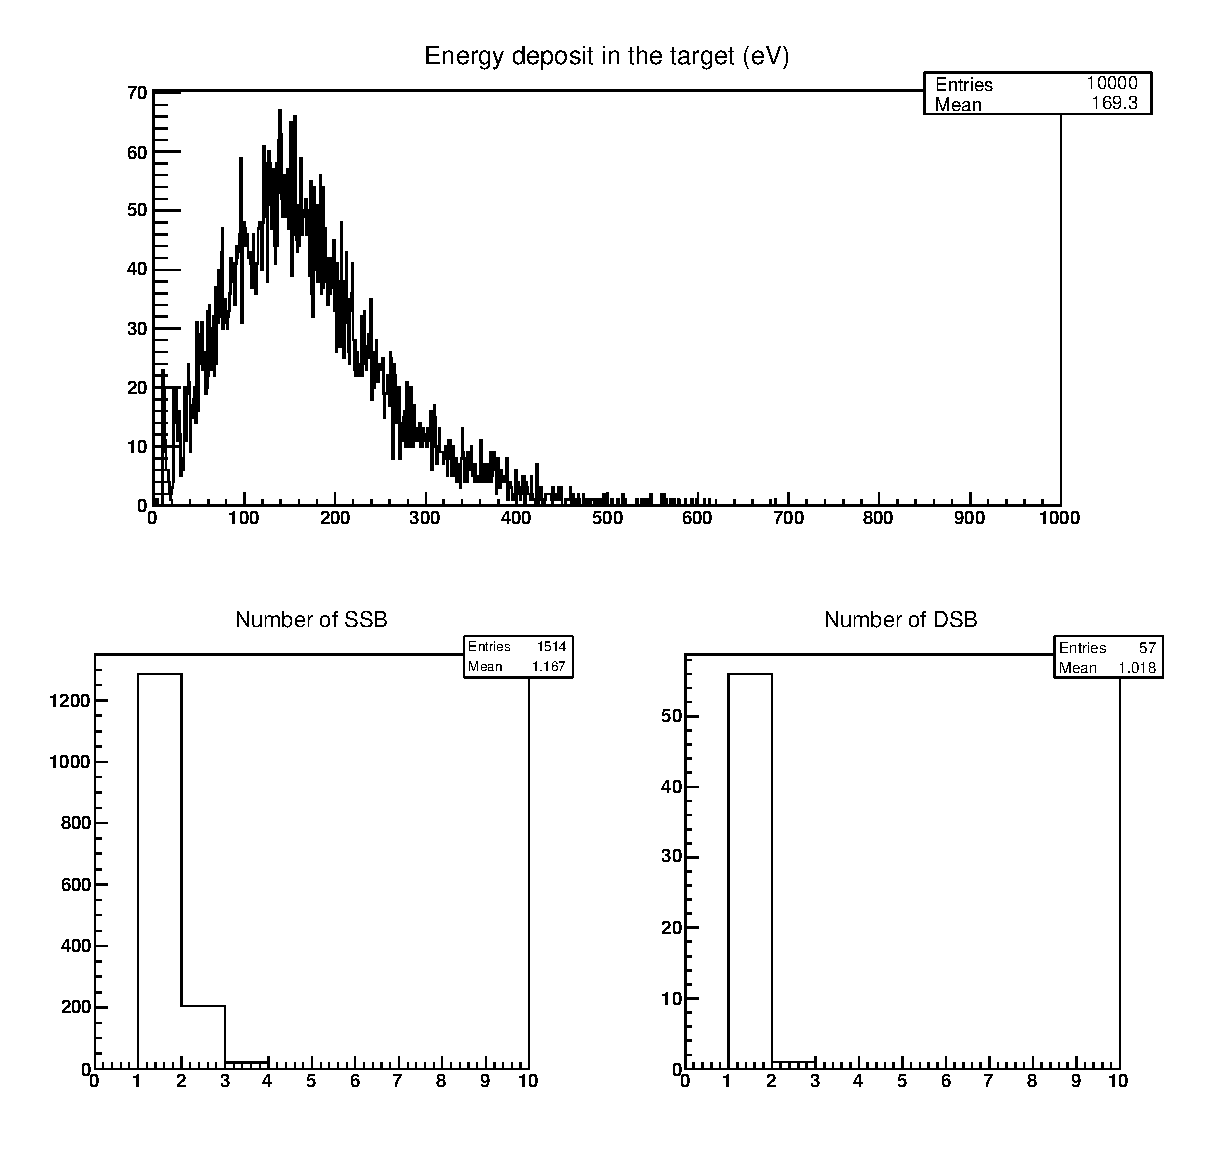
\includegraphics[width=.78\linewidth]{./Figures/proton1kev.eps}
  \caption{1 keV}
  \label{fig:sub5}
\end{subfigure}%
\begin{subfigure}{.5\textwidth}
  \centering
  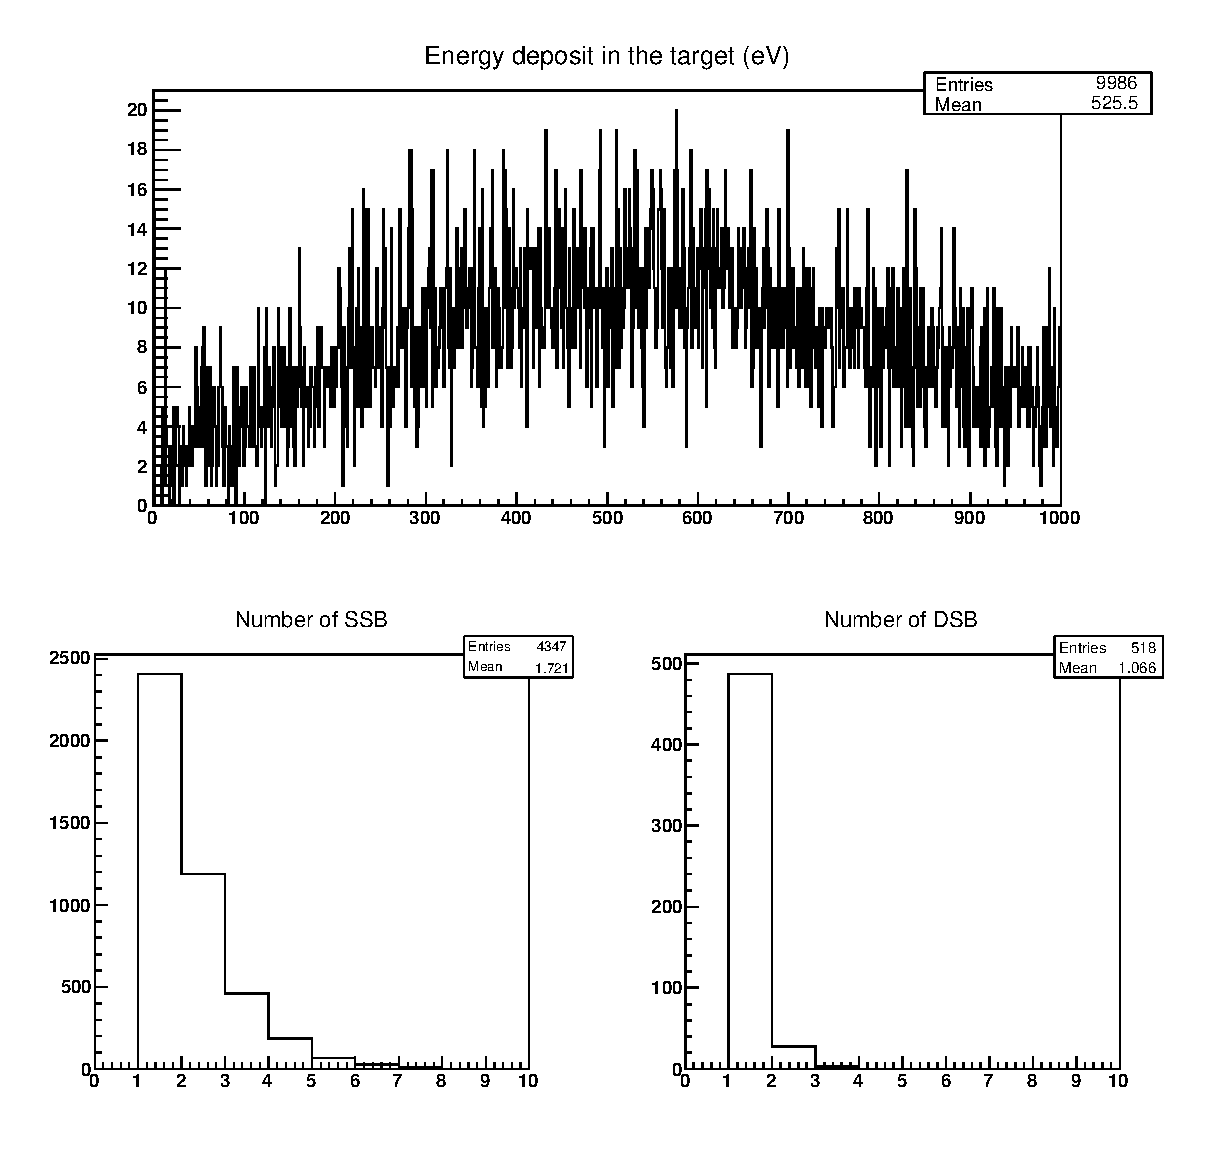
\includegraphics[width=.78\linewidth]{./Figures/proton200kev.eps}
  \caption{200 keV}
  \label{fig:sub6}
\end{subfigure}
\begin{subfigure}{.5\textwidth}
  \centering
  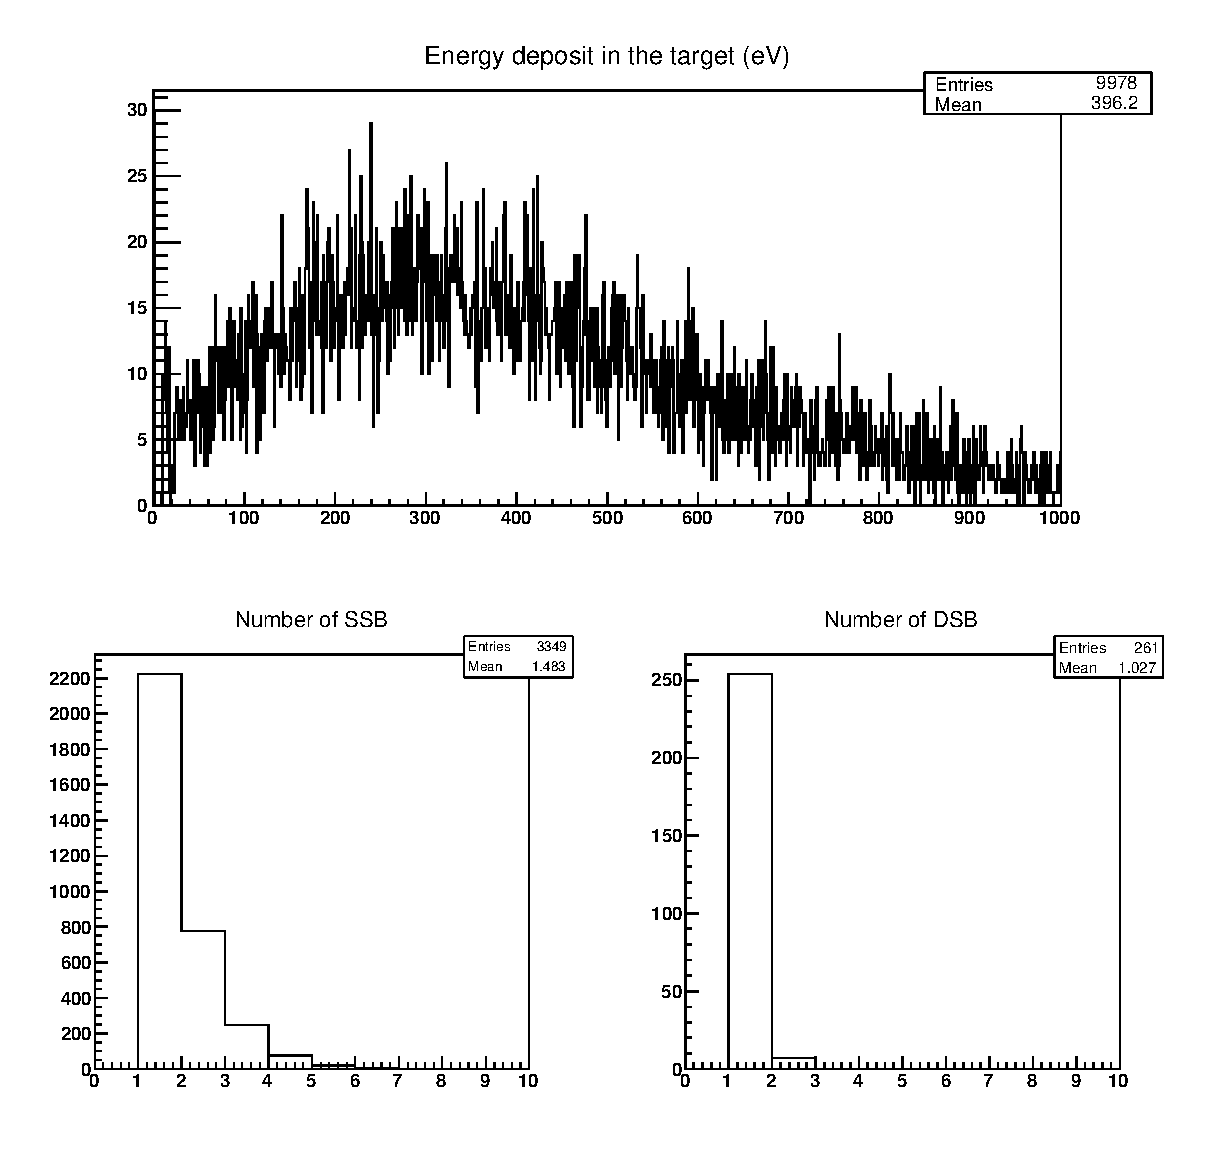
\includegraphics[width=.78\linewidth]{./Figures/proton400kev.eps}
  \caption{400 keV}
  \label{fig:sub7}
\end{subfigure}%
\begin{subfigure}{.5\textwidth}
  \centering
  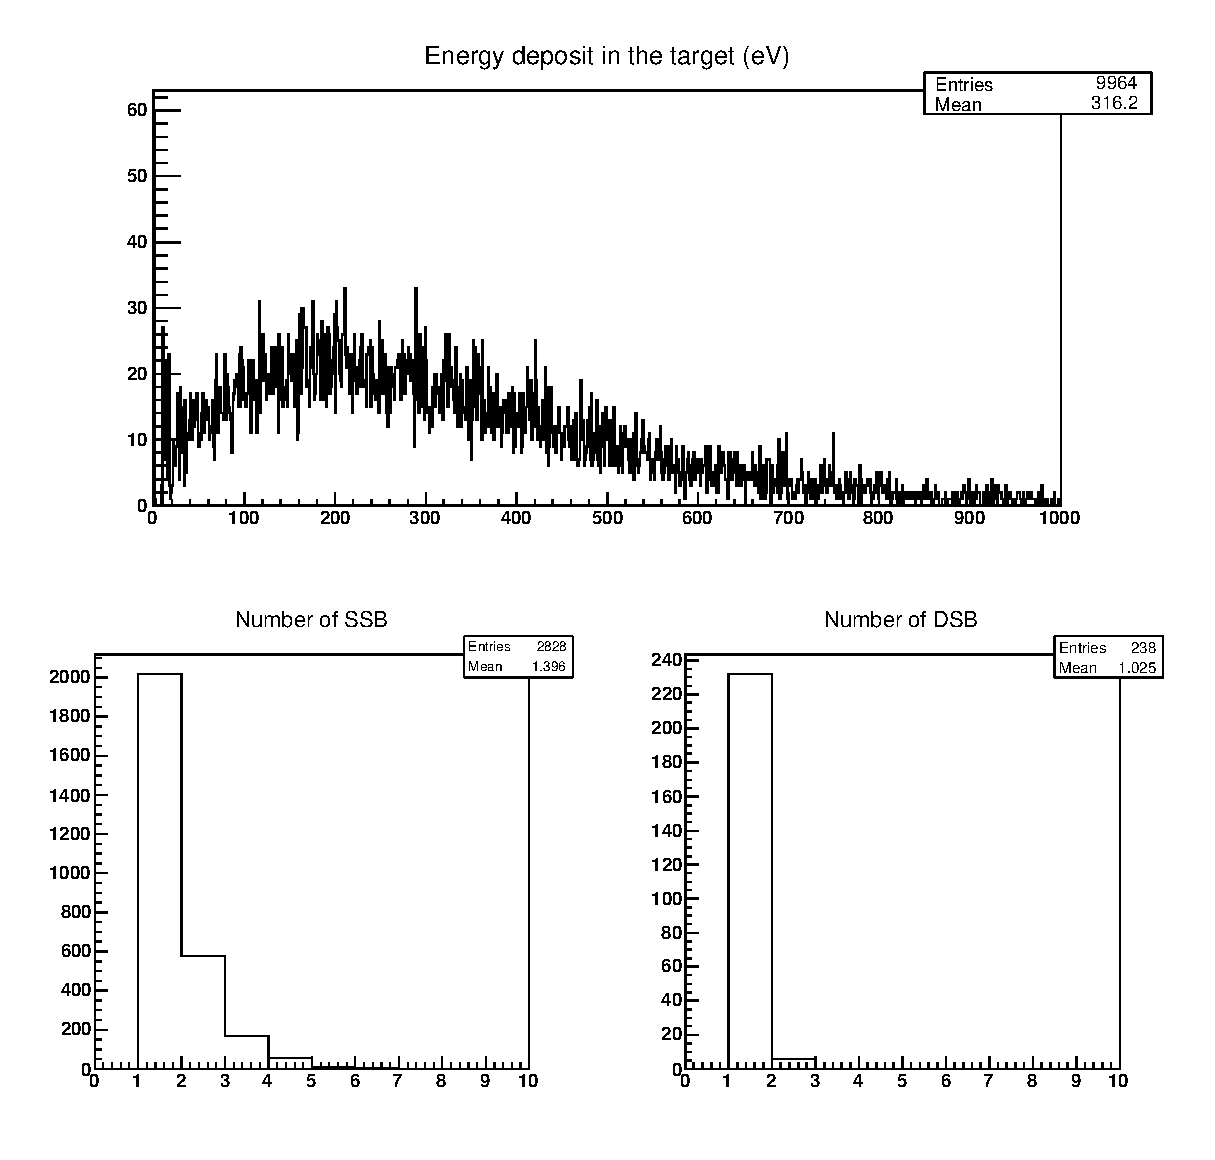
\includegraphics[width=.78\linewidth]{./Figures/proton600kev.eps}
  \caption{600 keV}
  \label{fig:sub8}
\end{subfigure}
\caption{Rompimientos simples y dobles para 1ZBB ($proton$)}
\label{fig:p}
\end{figure}



\begin{figure}
\centering
\begin{subfigure}{.5\textwidth}
  \centering
  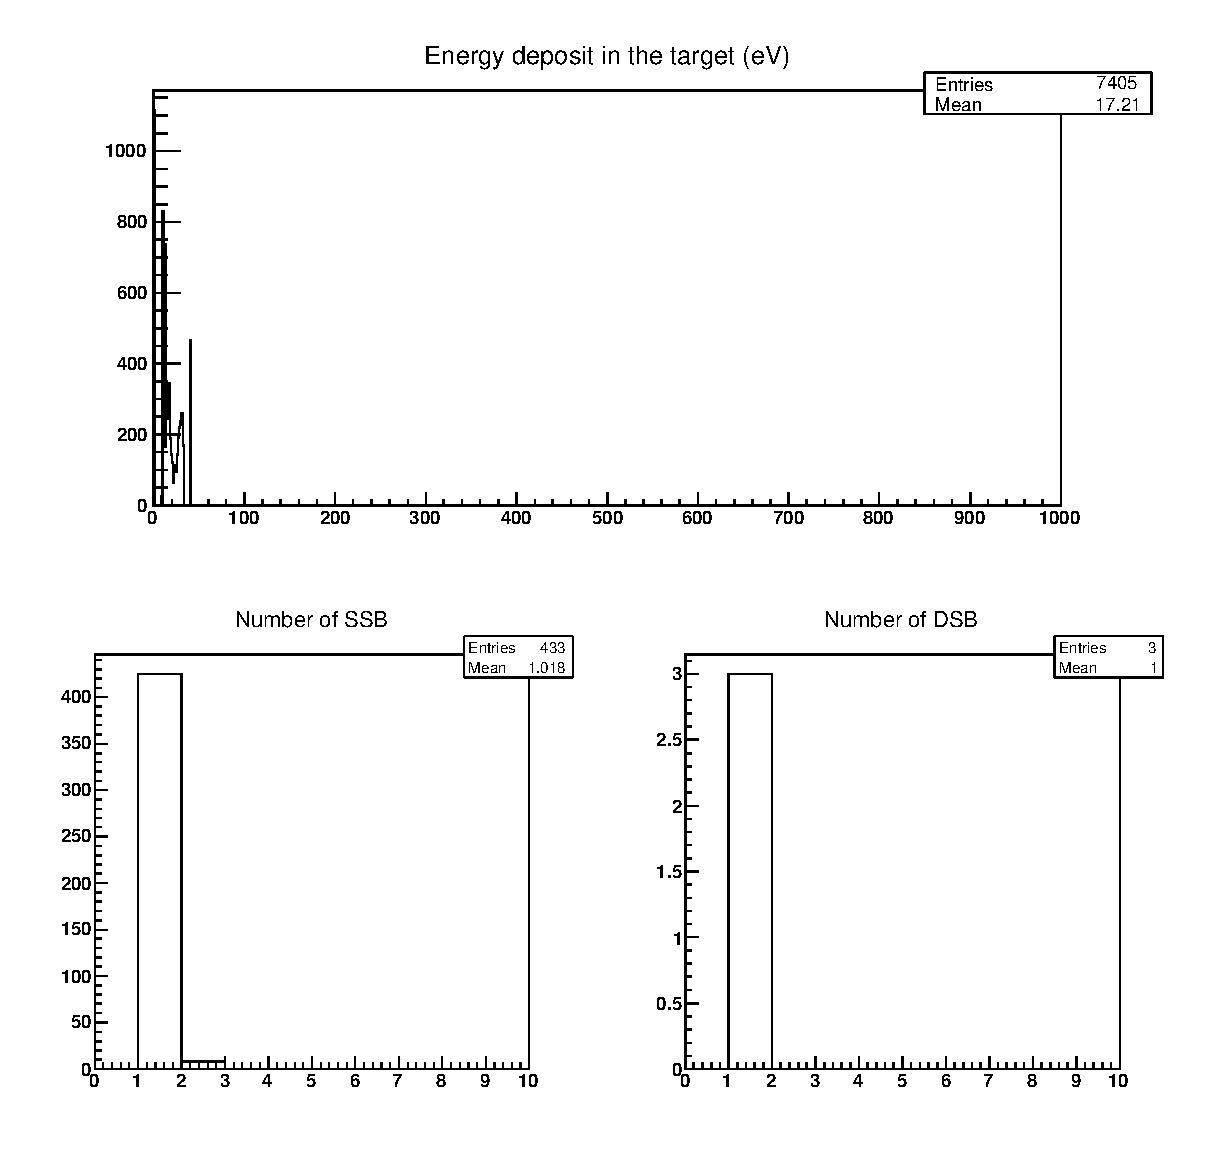
\includegraphics[width=.78\linewidth]{./Figures/040.eps}
  \caption{40 eV}
  \label{fig:sube1}
\end{subfigure}%
\begin{subfigure}{.5\textwidth}
  \centering
  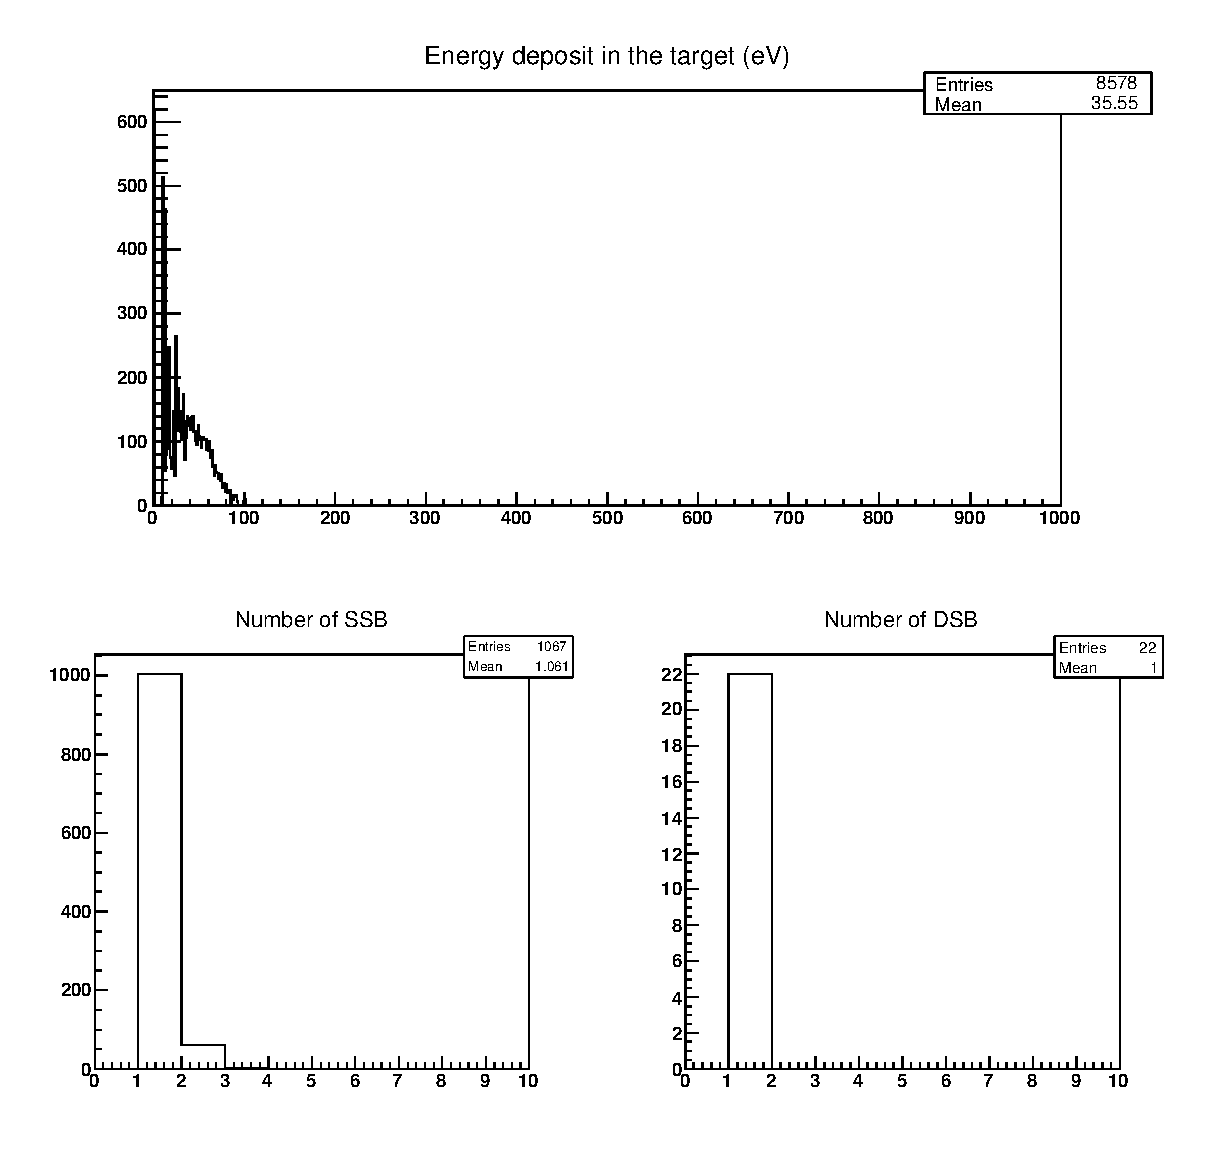
\includegraphics[width=.78\linewidth]{./Figures/1.eps}
  \caption{100 eV}
  \label{fig:sube2}
\end{subfigure}
\begin{subfigure}{.5\textwidth}
  \centering
  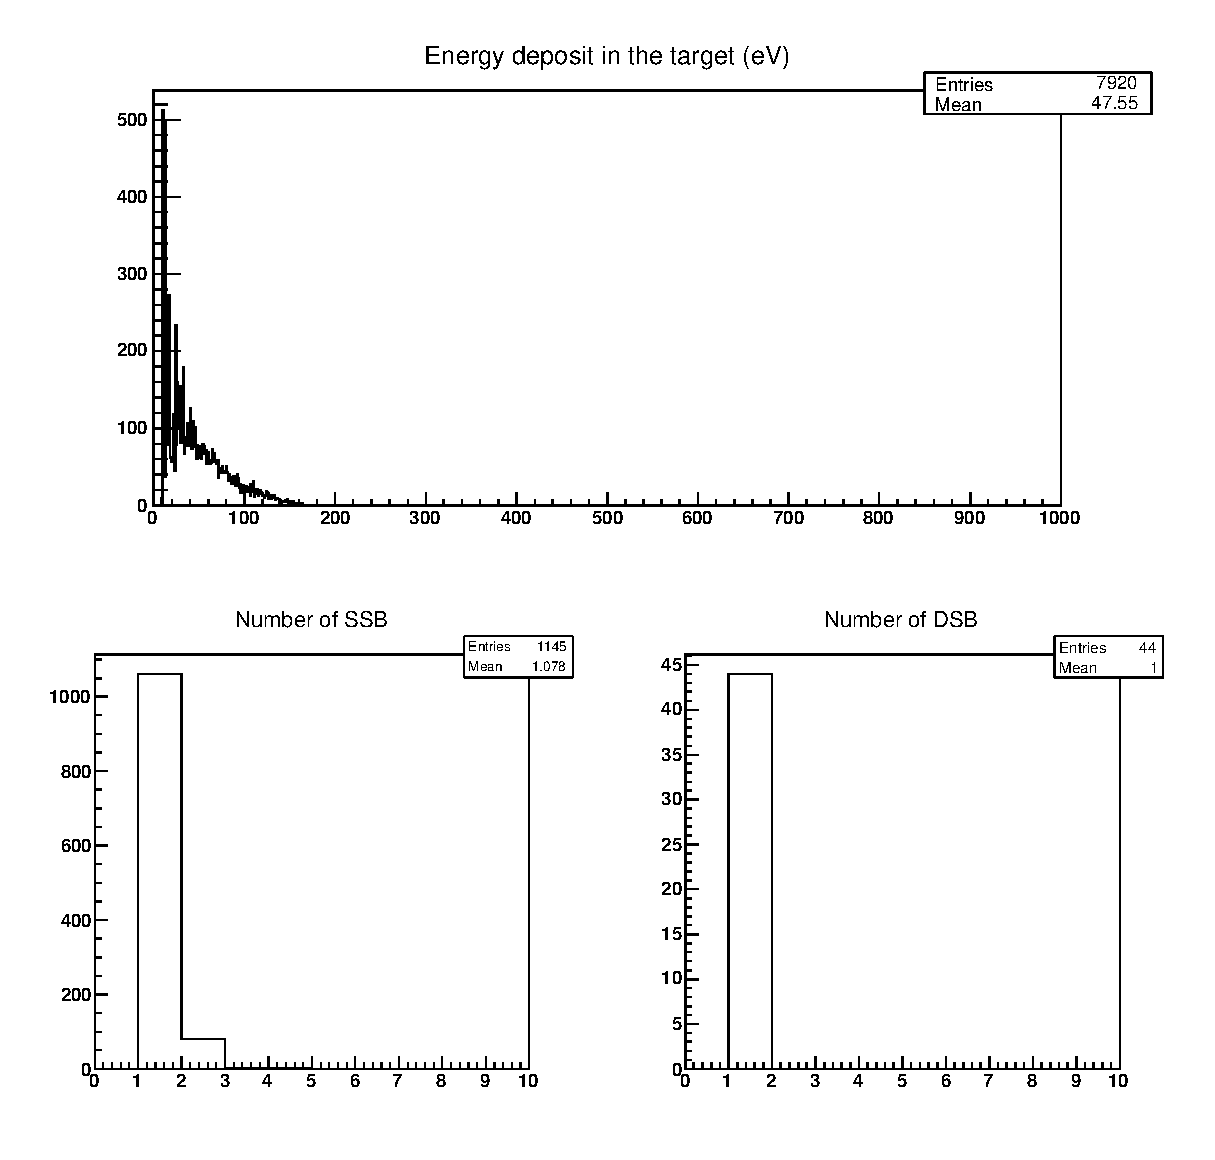
\includegraphics[width=.78\linewidth]{./Figures/2.eps}
  \caption{200 eV}
  \label{fig:sube3}
\end{subfigure}%
\begin{subfigure}{.5\textwidth}
  \centering
  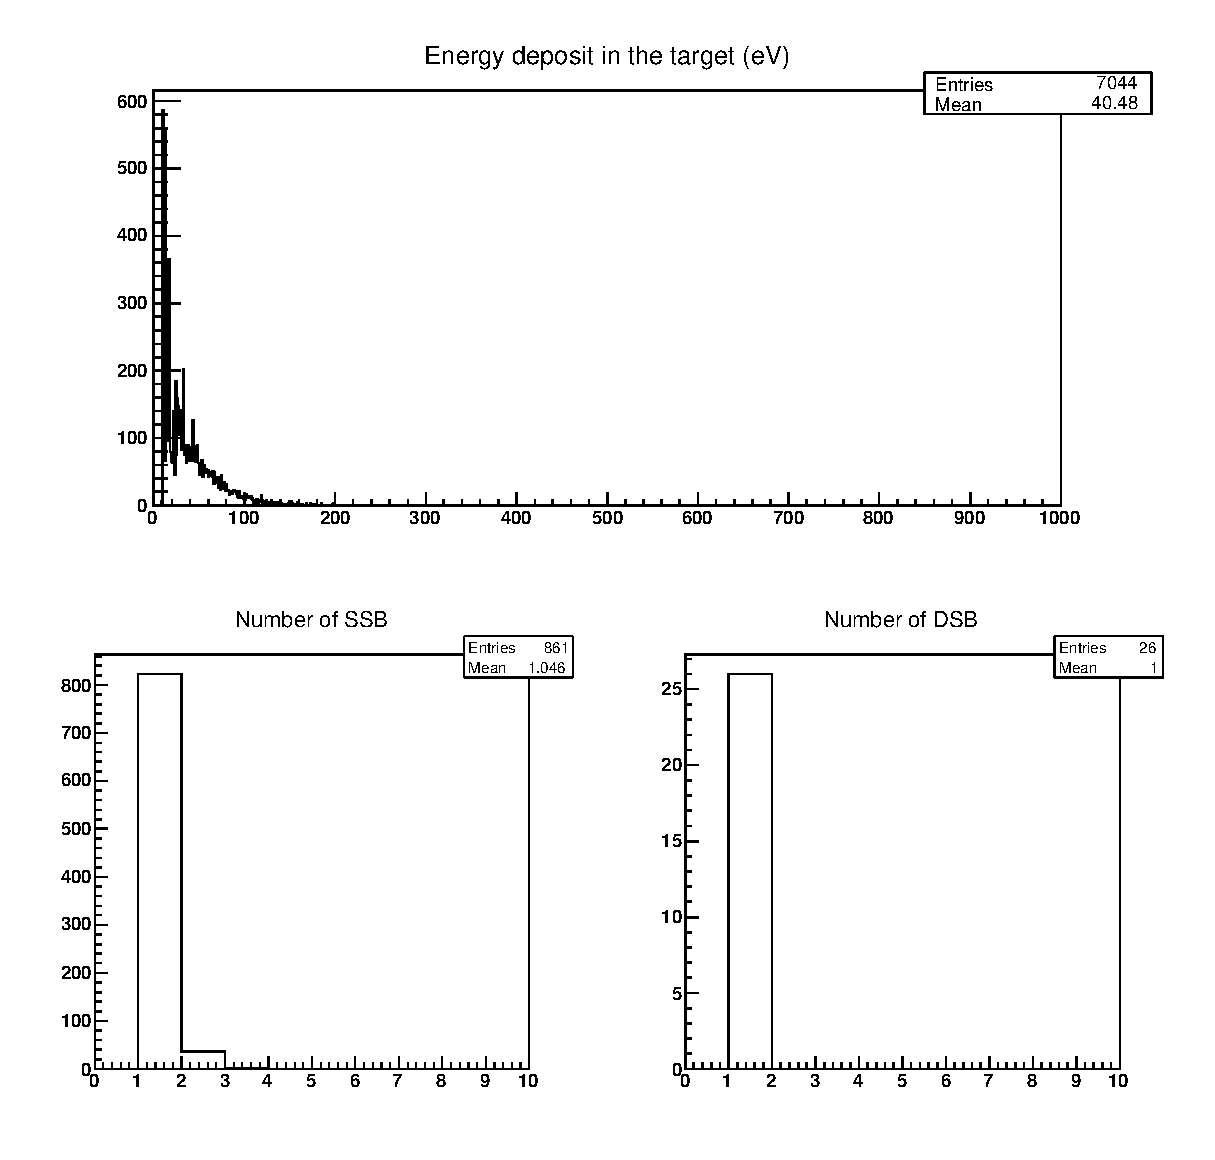
\includegraphics[width=.78\linewidth]{./Figures/3.eps}
  \caption{400 eV}
  \label{fig:sube4}
\end{subfigure}
\begin{subfigure}{.5\textwidth}
  \centering
  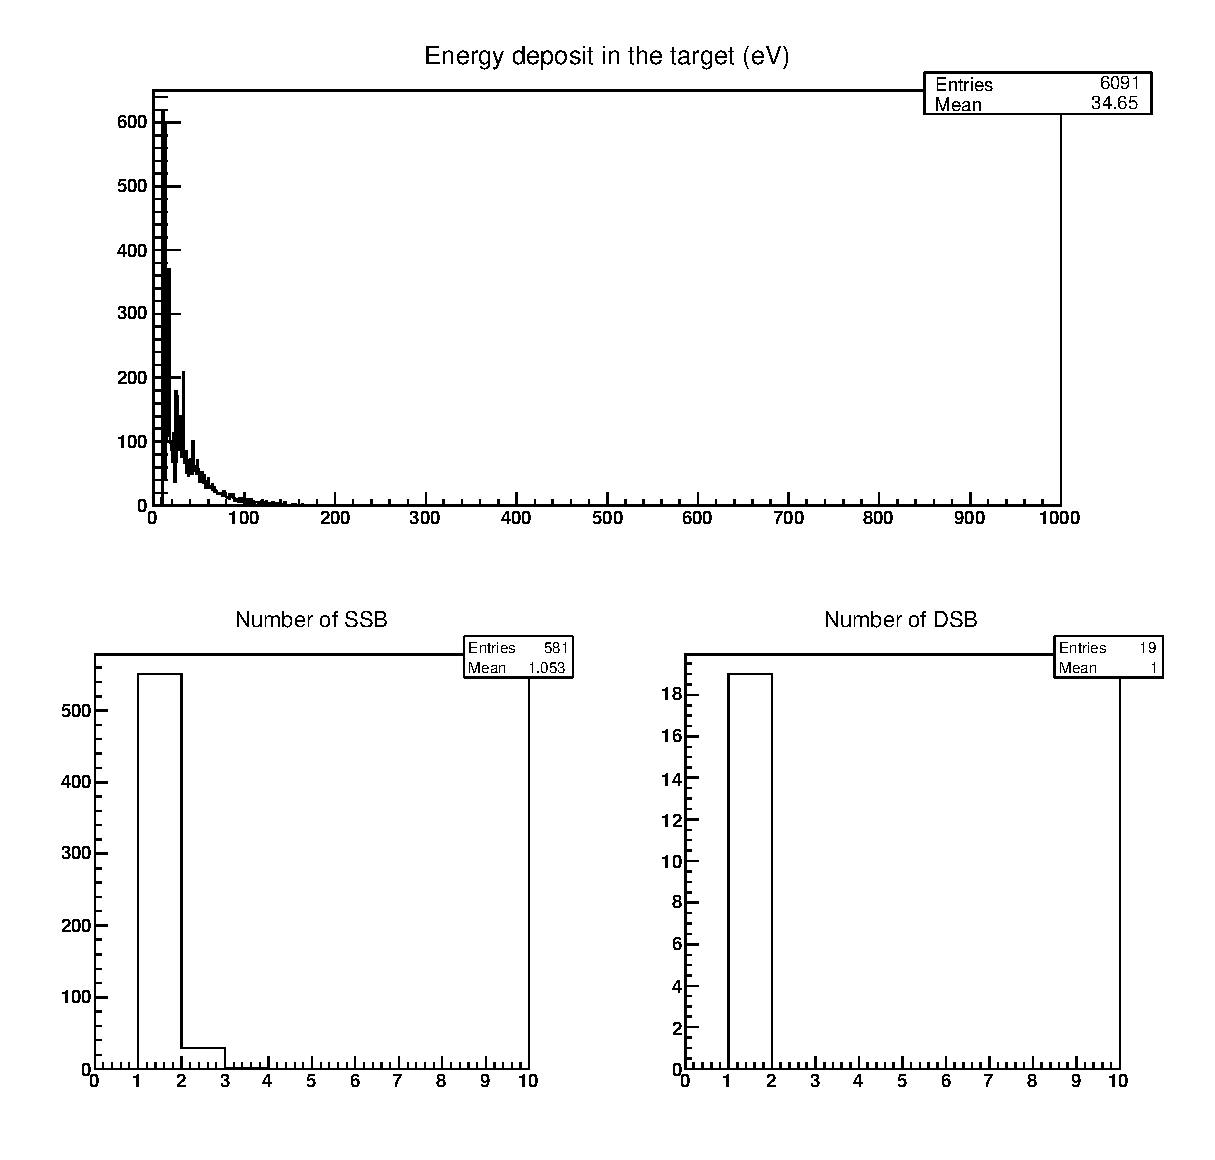
\includegraphics[width=.78\linewidth]{./Figures/4.eps}
  \caption{600 eV}
  \label{fig:sube5}
\end{subfigure}%
\begin{subfigure}{.5\textwidth}
  \centering
  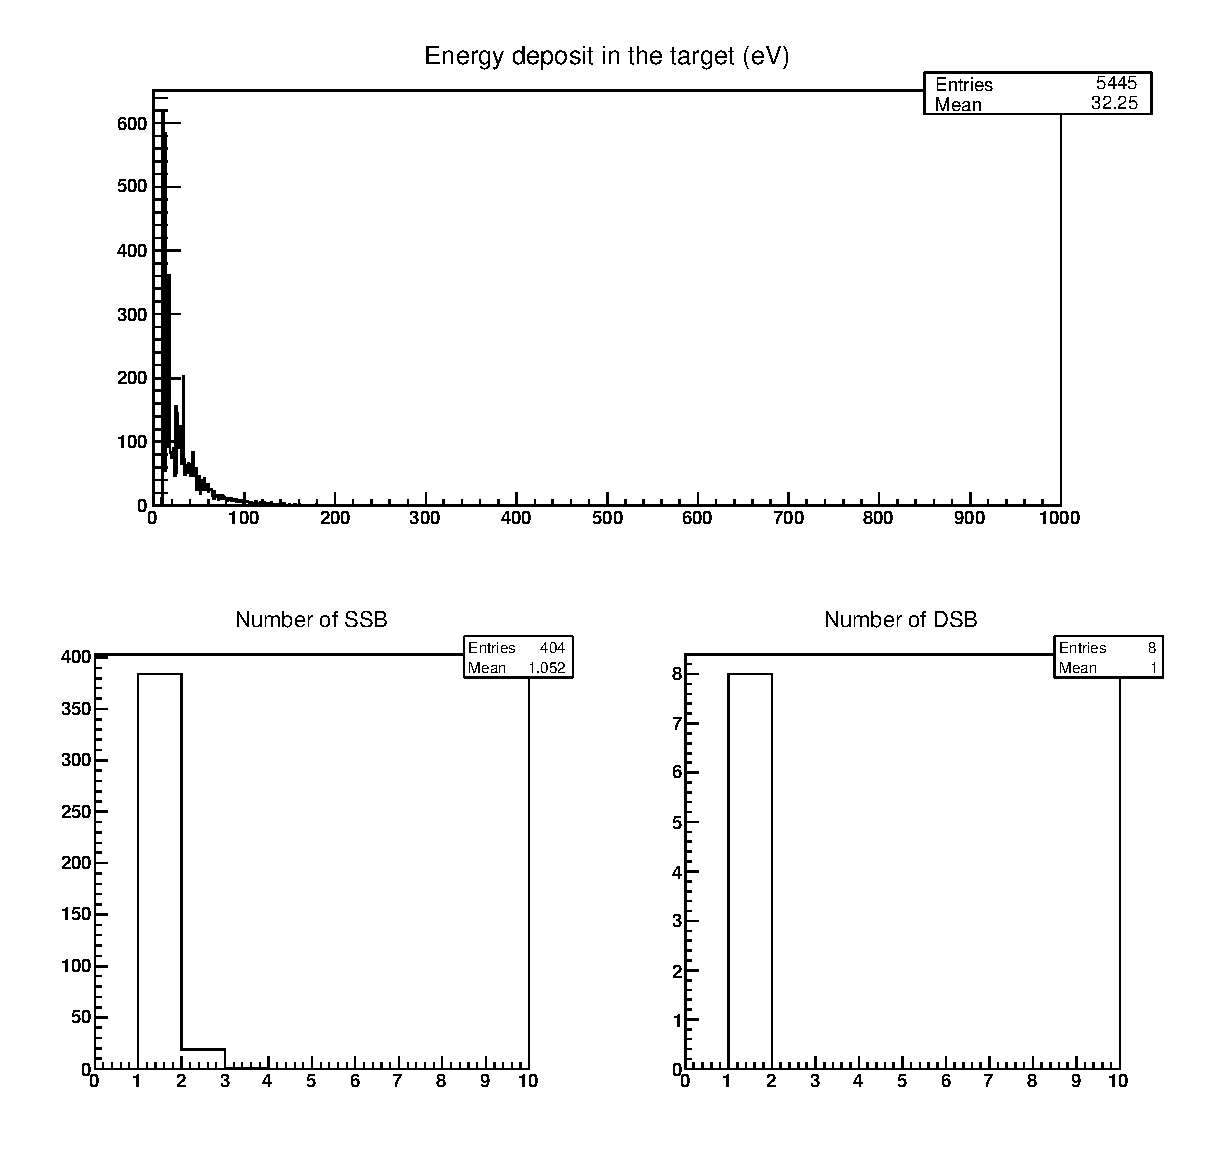
\includegraphics[width=.78\linewidth]{./Figures/5.eps}
  \caption{800 eV}
  \label{fig:sube6}
\end{subfigure}
\begin{subfigure}{.5\textwidth}
  \centering
  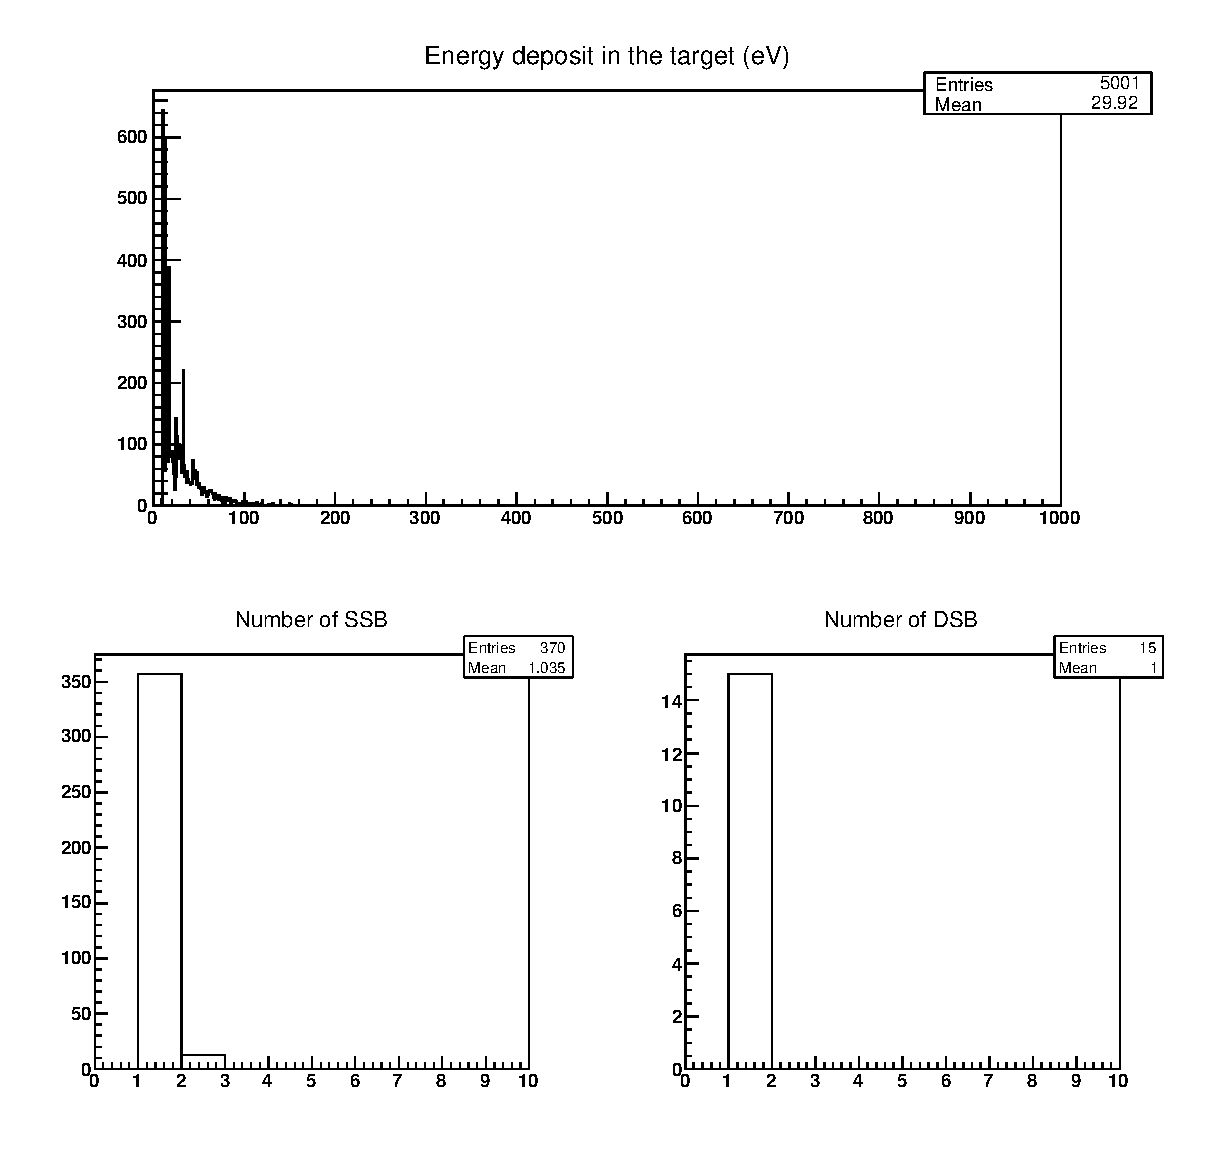
\includegraphics[width=.78\linewidth]{./Figures/6.eps}
  \caption{1 keV}
  \label{fig:sube7}
\end{subfigure}%
\begin{subfigure}{.5\textwidth}
  \centering
  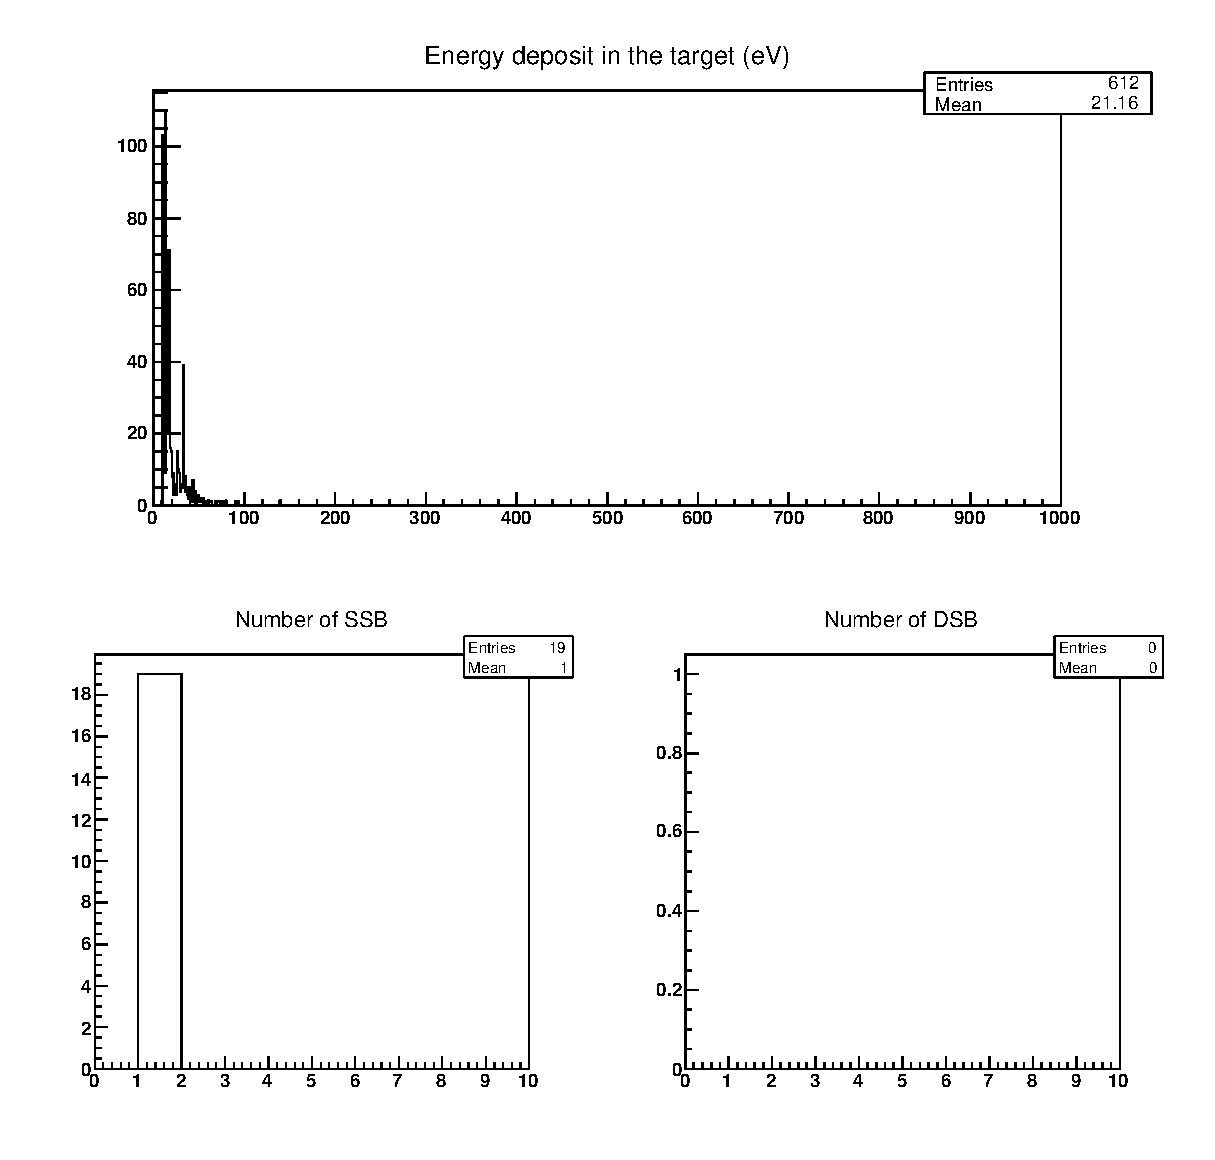
\includegraphics[width=.78\linewidth]{./Figures/7.eps}
  \caption{20 keV}
  \label{fig:sube8}
\end{subfigure}
\caption{Rompimientos simples y dobles para 1FZX ($e-$)}
\label{fig:e2}
\end{figure}




\begin{figure}
\centering
\begin{subfigure}{.5\textwidth}
  \centering
  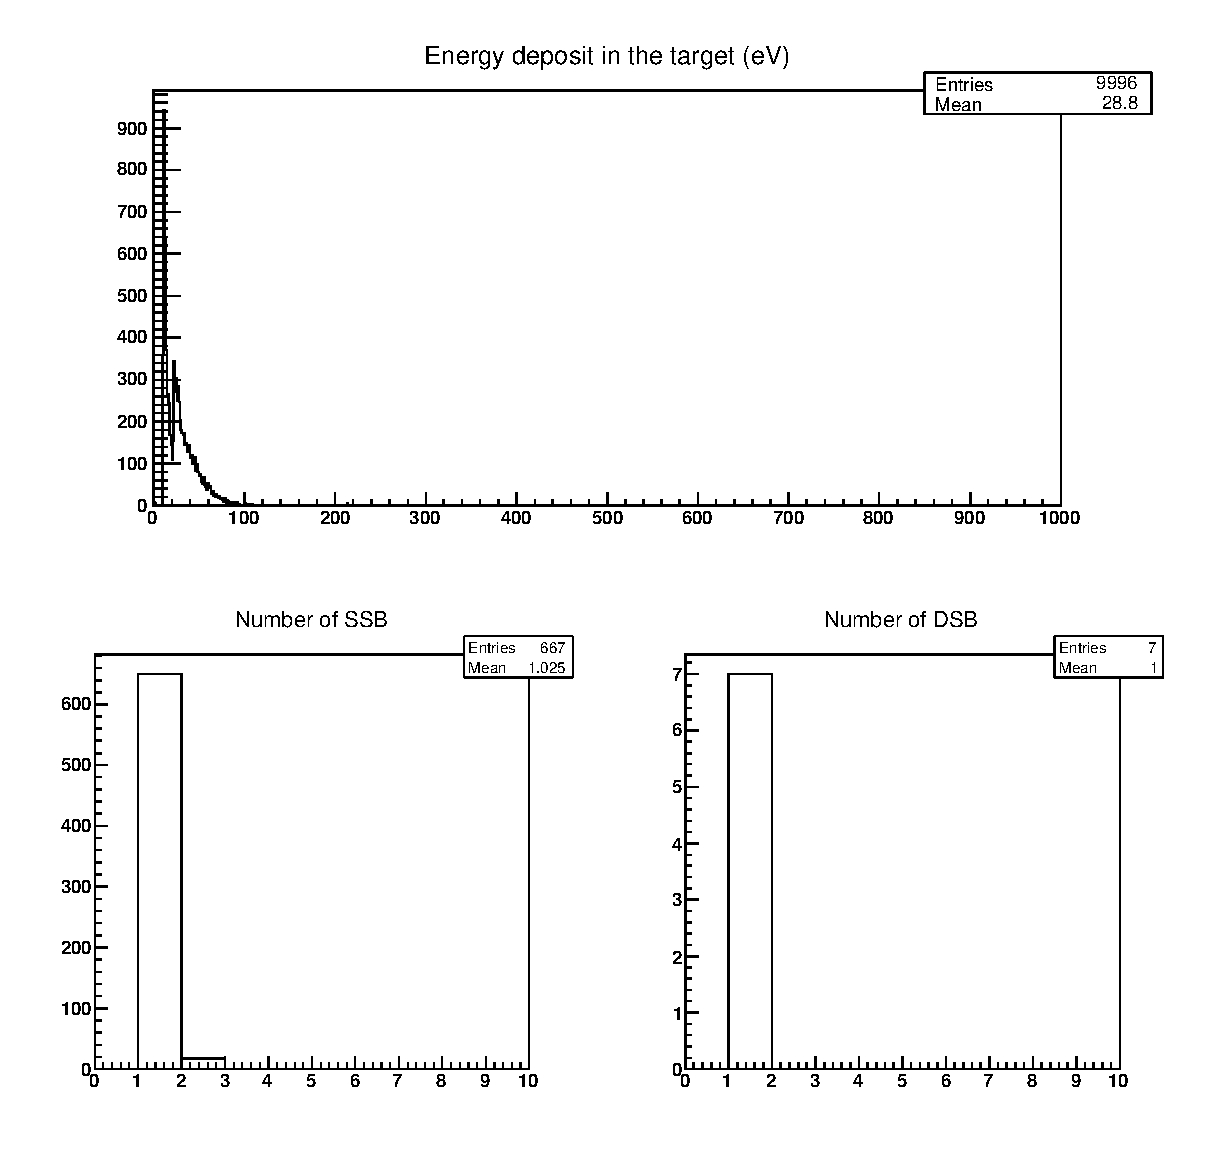
\includegraphics[width=.78\linewidth]{./Figures/11.eps}
  \caption{200 eV}
  \label{fig:subi1}
\end{subfigure}%
\begin{subfigure}{.5\textwidth}
  \centering
  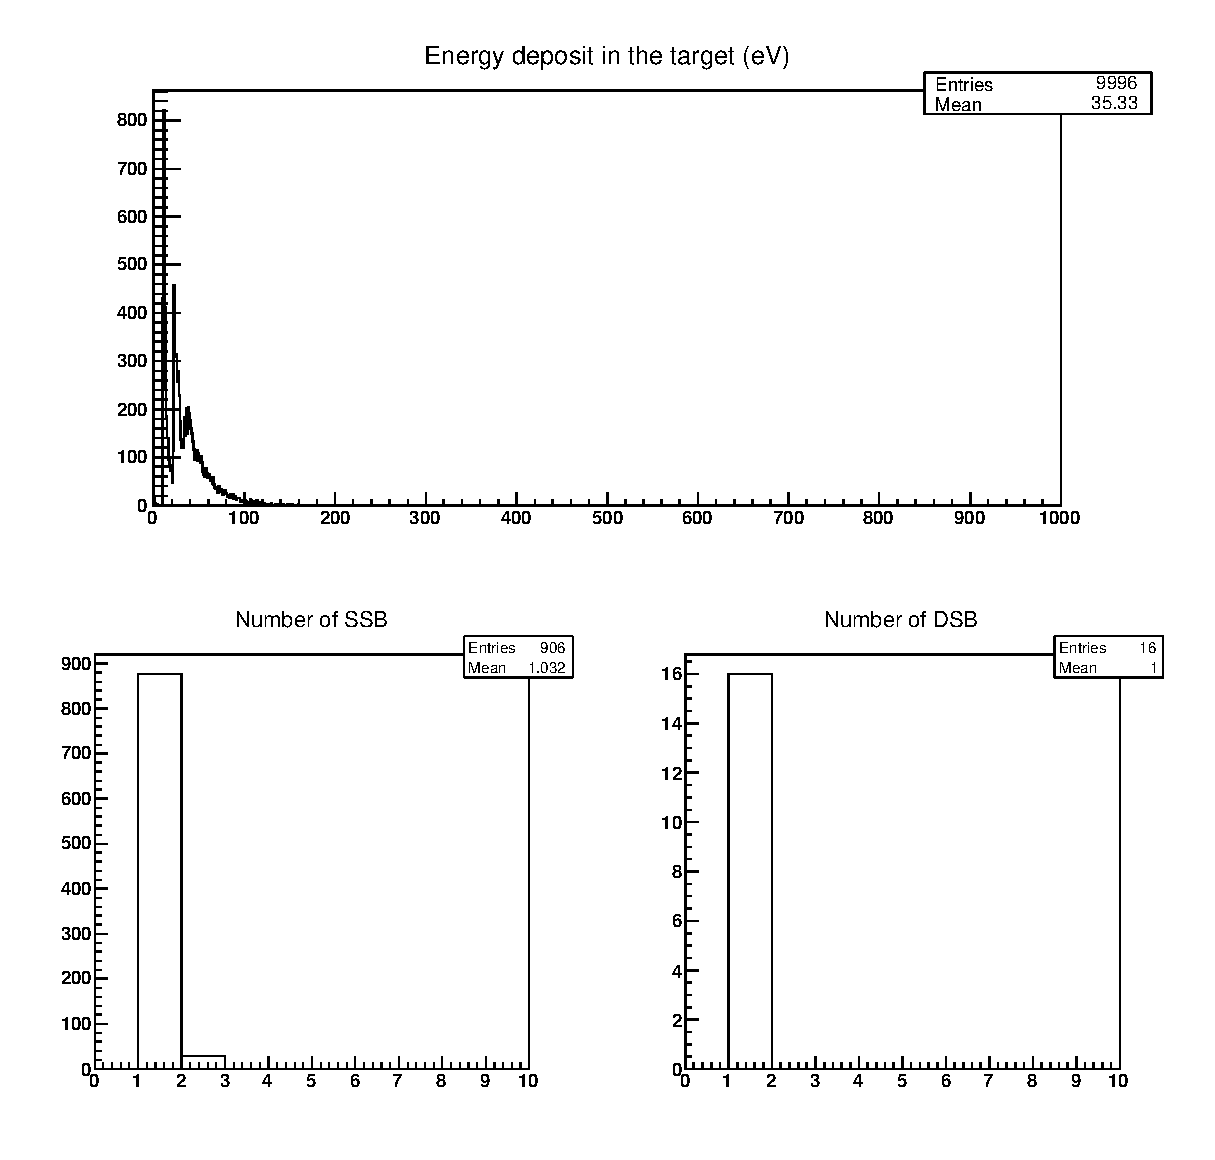
\includegraphics[width=.78\linewidth]{./Figures/22.eps}
  \caption{400 eV}
  \label{fig:subi2}
\end{subfigure}
\begin{subfigure}{.5\textwidth}
  \centering
  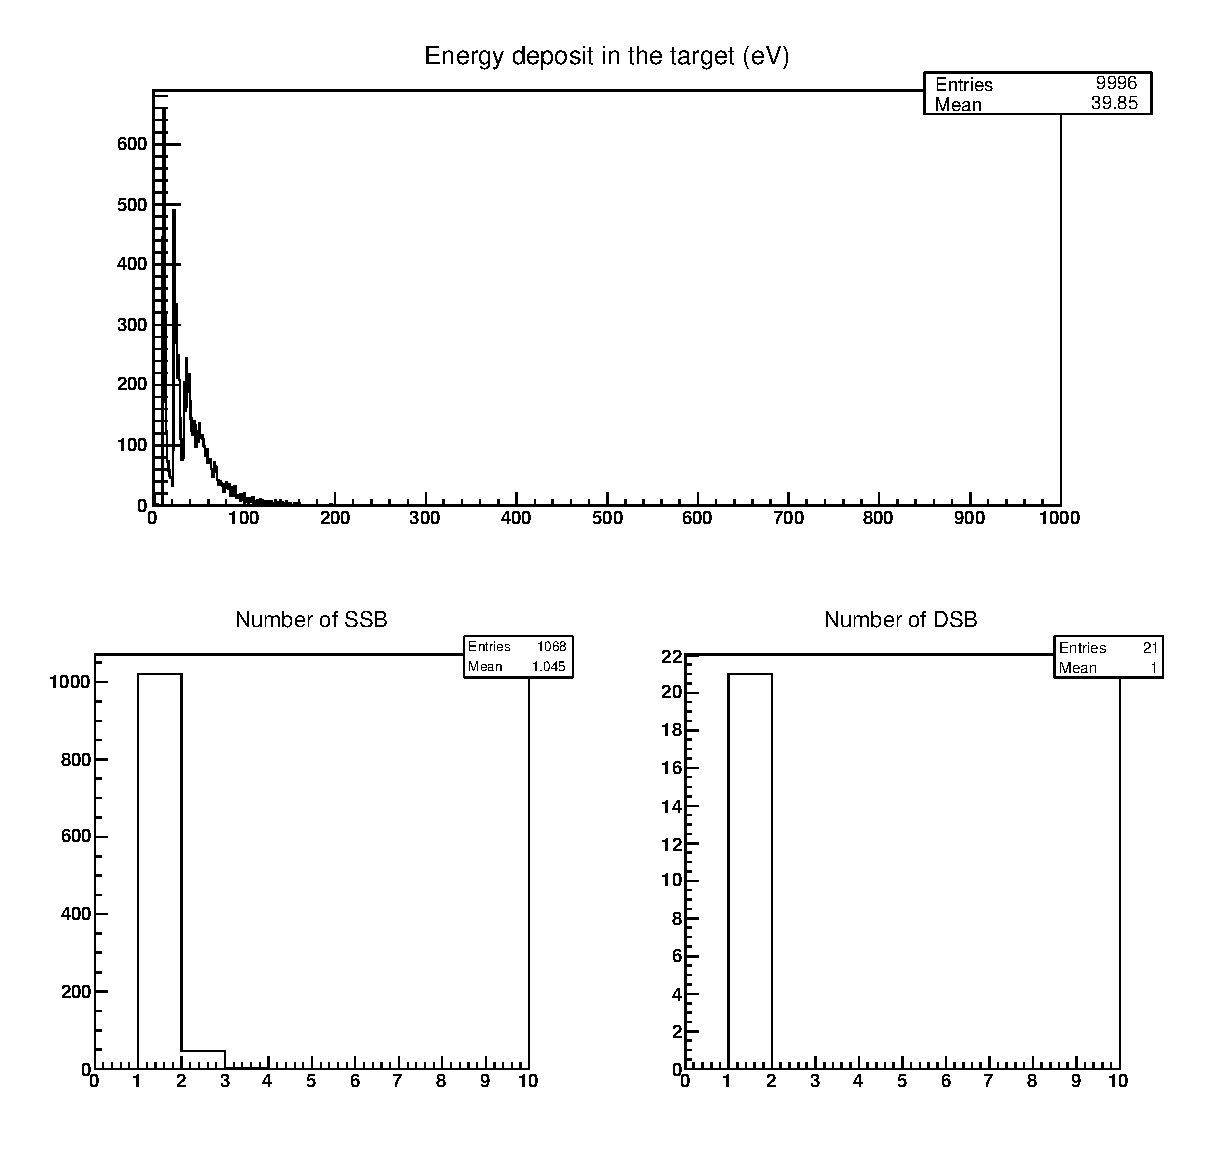
\includegraphics[width=.78\linewidth]{./Figures/33.eps}
  \caption{600 eV}
  \label{fig:subi3}
\end{subfigure}%
\begin{subfigure}{.5\textwidth}
  \centering
  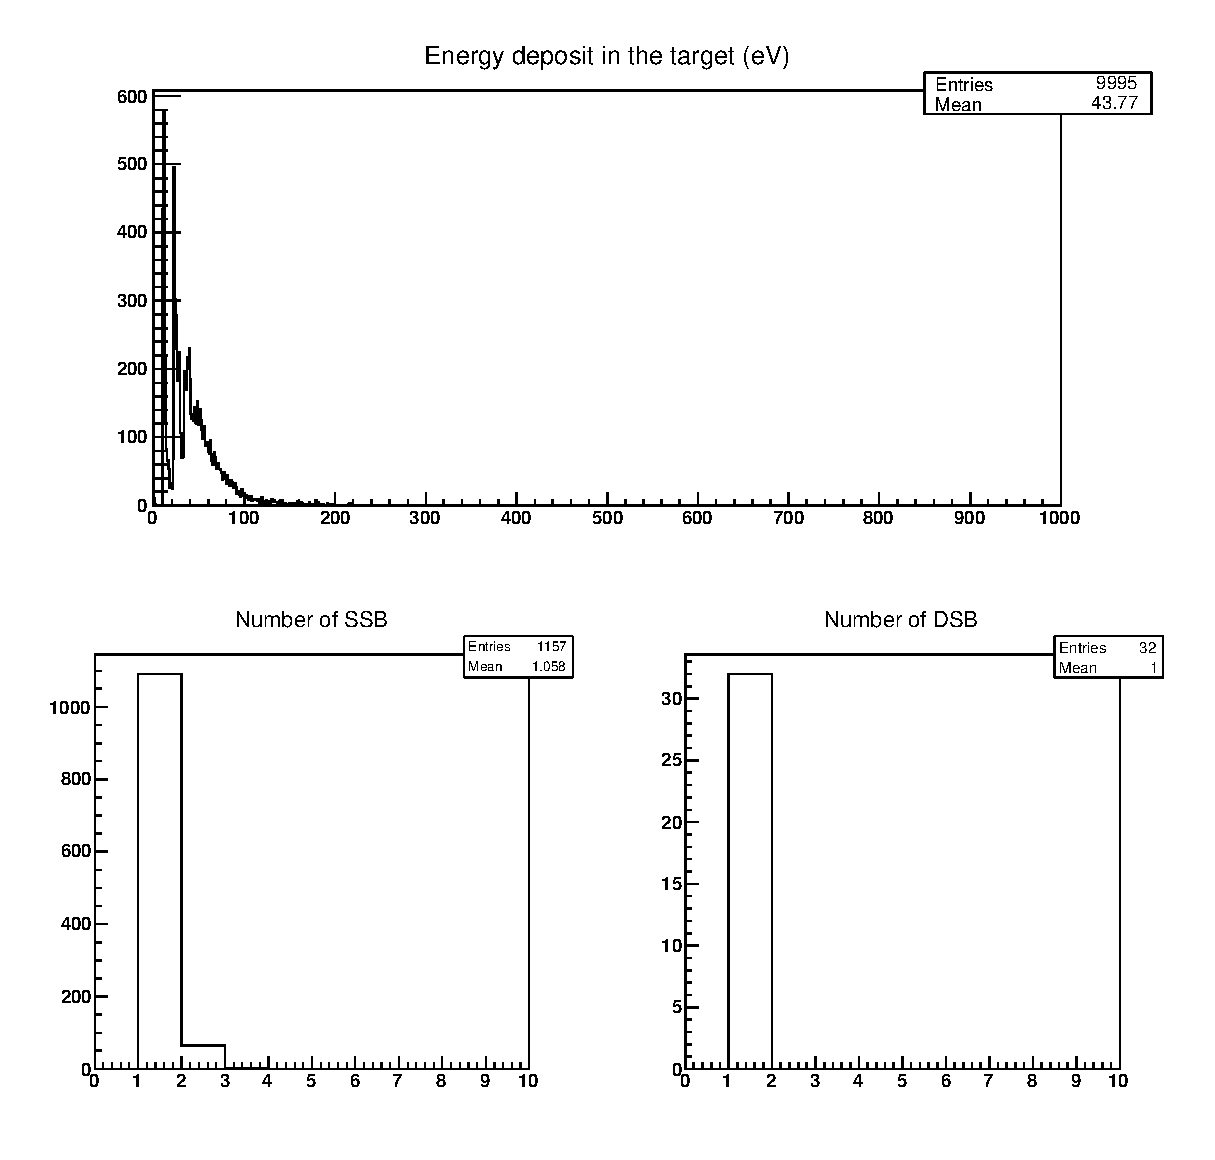
\includegraphics[width=.78\linewidth]{./Figures/44.eps}
  \caption{800 eV}
  \label{fig:subi4}
\end{subfigure}
\begin{subfigure}{.5\textwidth}
  \centering
  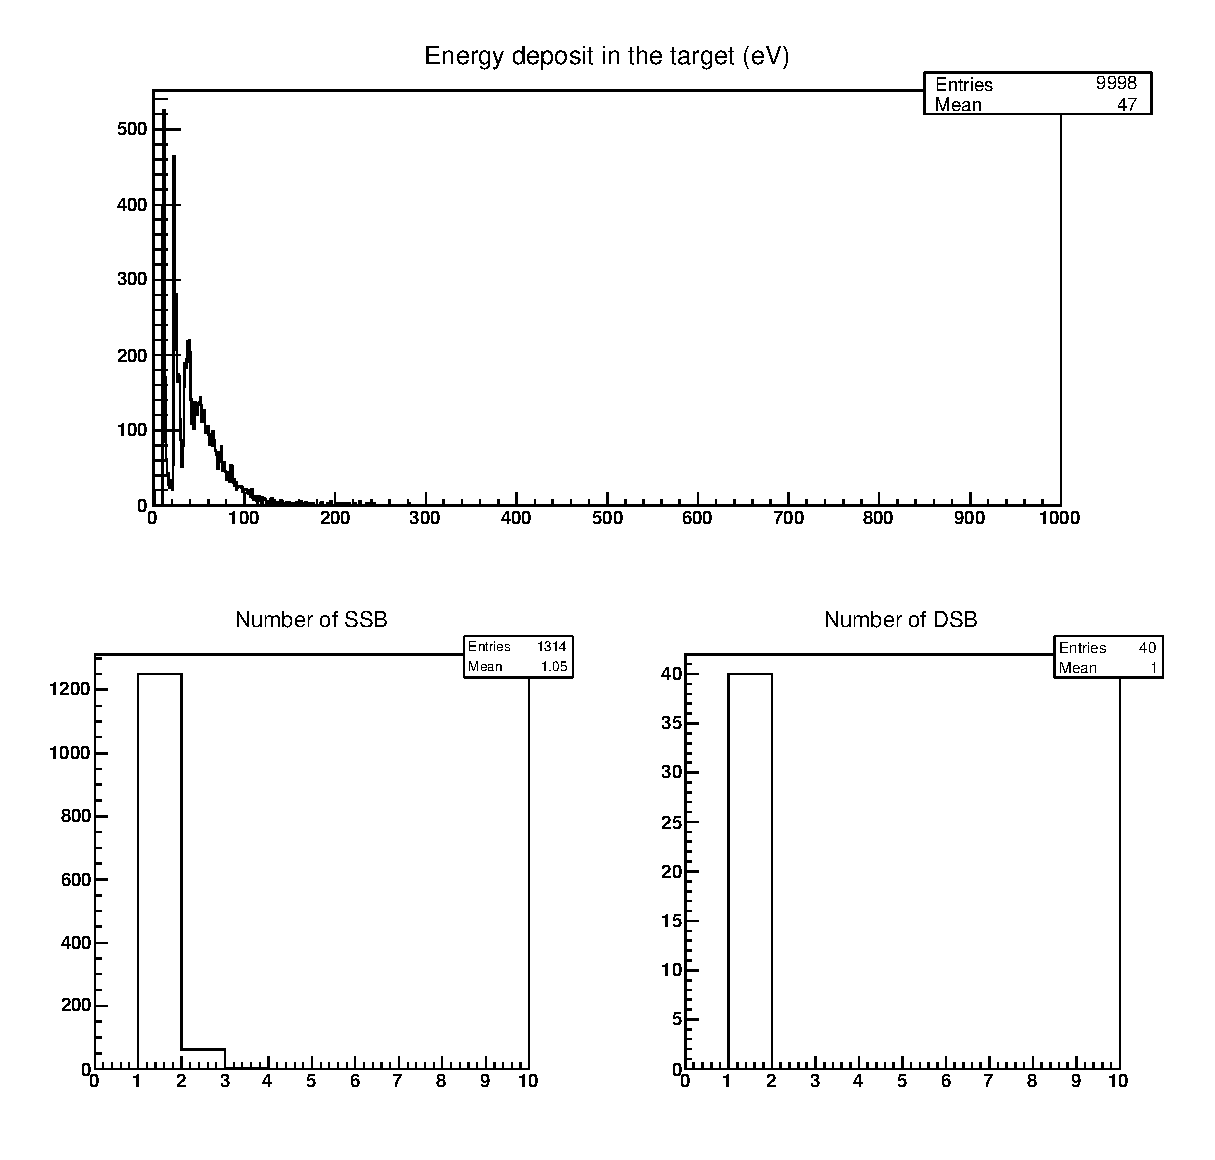
\includegraphics[width=.78\linewidth]{./Figures/55.eps}
  \caption{1 keV}
  \label{fig:subi5}
\end{subfigure}%
\begin{subfigure}{.5\textwidth}
  \centering
  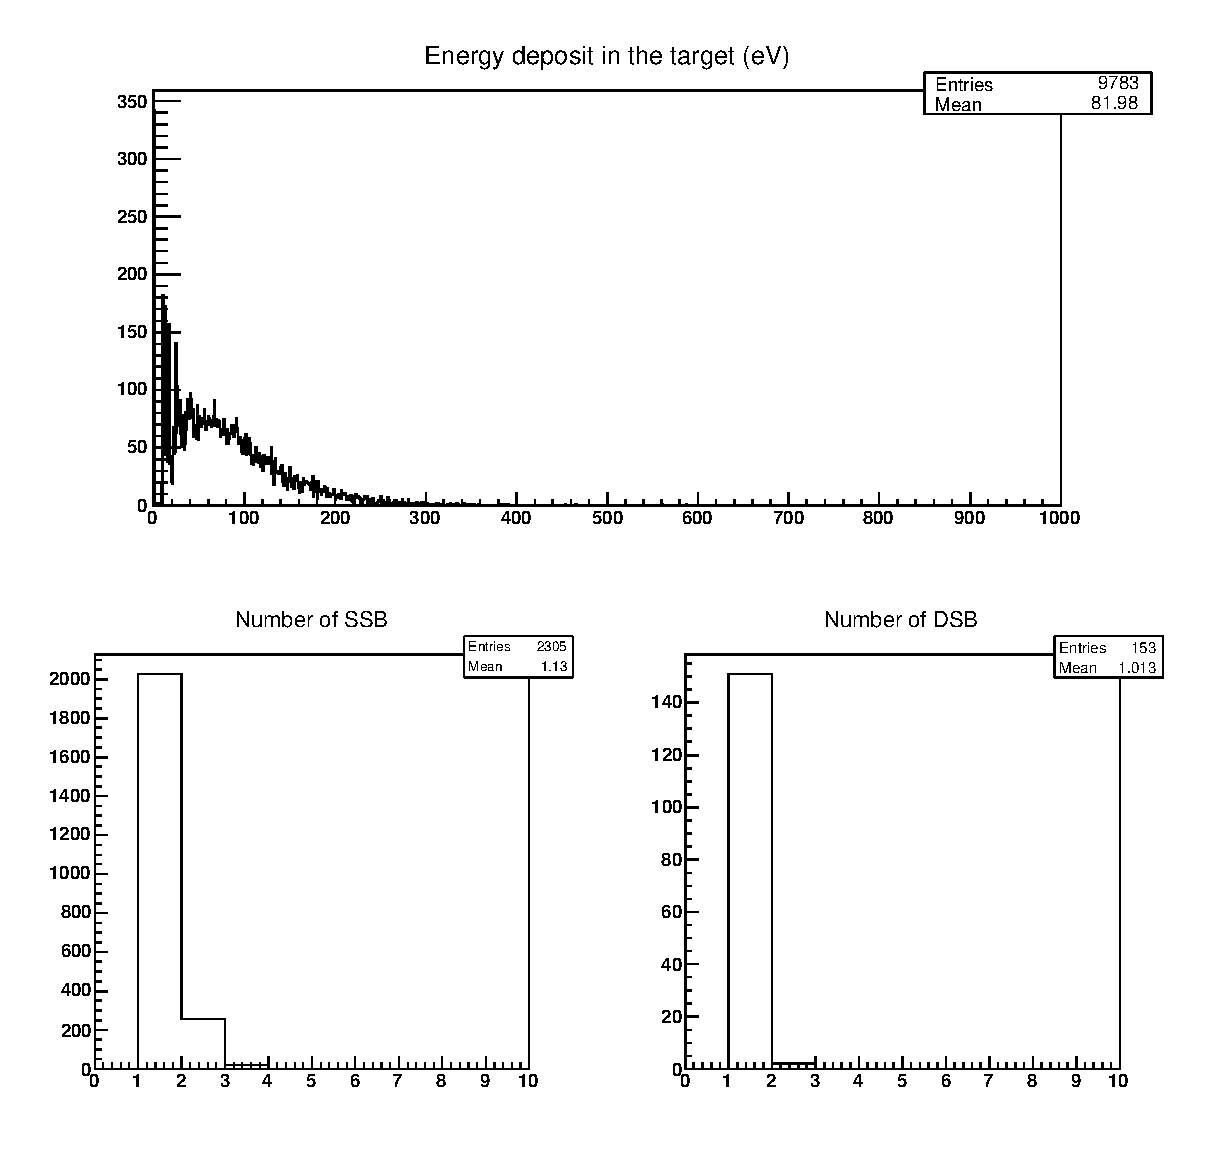
\includegraphics[width=.78\linewidth]{./Figures/66.eps}
  \caption{200 keV}
  \label{fig:subi6}
\end{subfigure}
\begin{subfigure}{.5\textwidth}
  \centering
  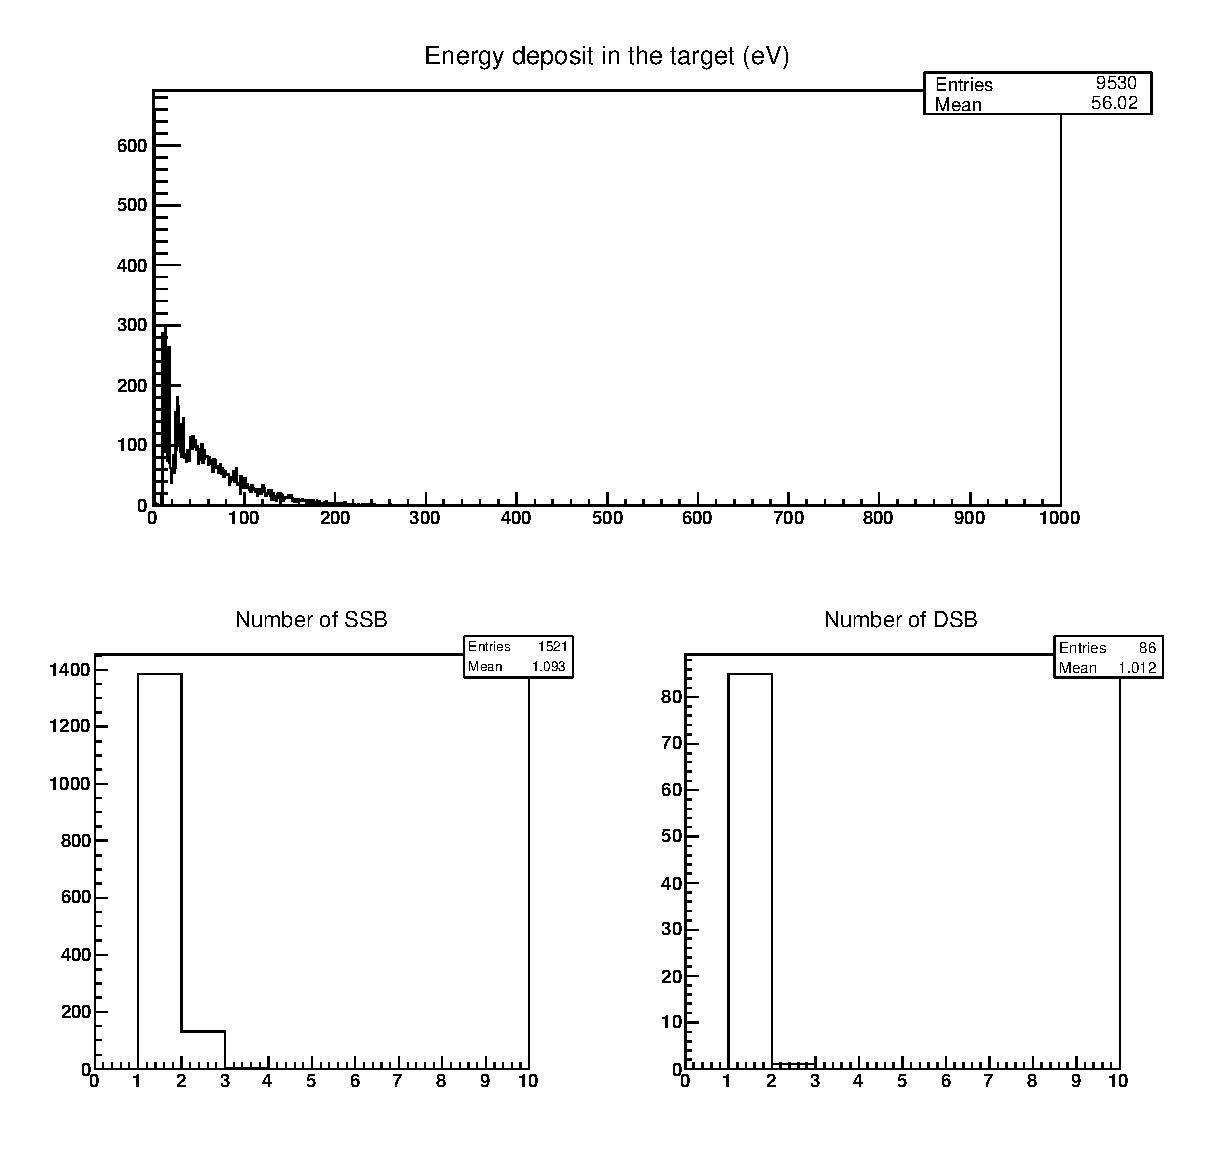
\includegraphics[width=.78\linewidth]{./Figures/77.eps}
  \caption{400 keV}
  \label{fig:subi7}
\end{subfigure}%
\begin{subfigure}{.5\textwidth}
  \centering
  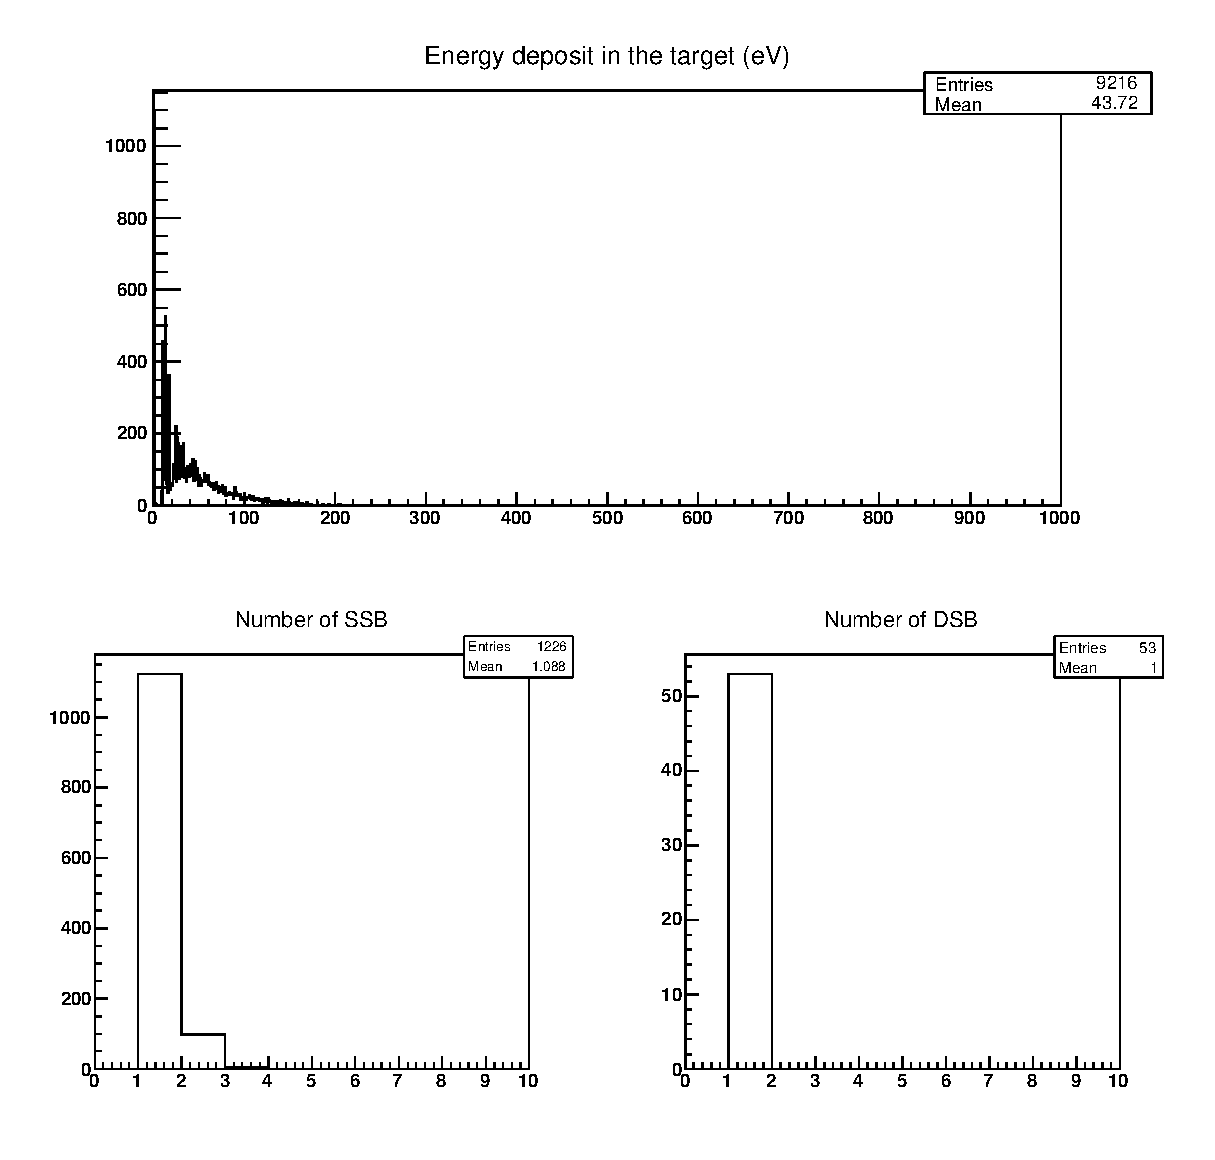
\includegraphics[width=.78\linewidth]{./Figures/88.eps}
  \caption{600 keV}
  \label{fig:subi8}
\end{subfigure}
\caption{Rompimientos simples y dobles para 1FZX ($proton$)}
\label{fig:p2}
\end{figure}




\begin{figure}
\centering
\begin{subfigure}{.5\textwidth}
  \centering
  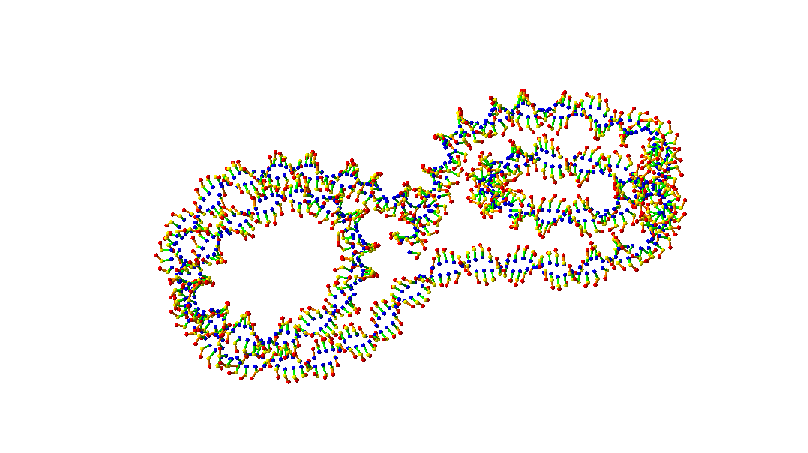
\includegraphics[width=.78\linewidth]{./Figures/baresi.png}
  \caption{Baricentro residuos }
  \label{fig:sub11}
\end{subfigure}%
\begin{subfigure}{.5\textwidth}
  \centering
  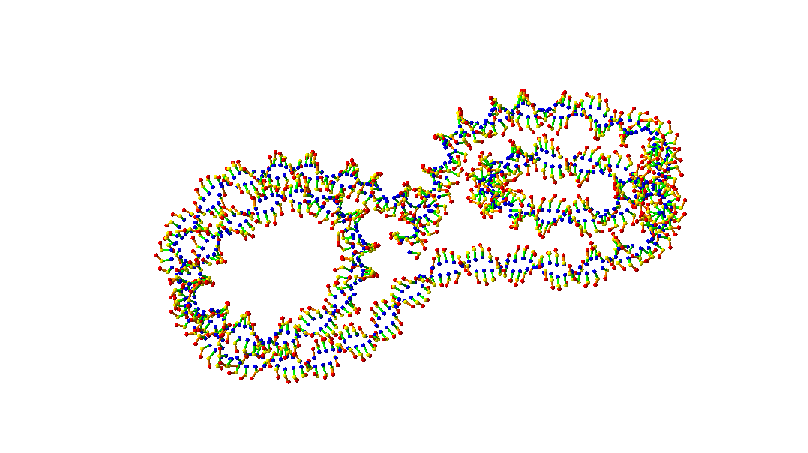
\includegraphics[width=.78\linewidth]{./Figures/baresi.png}
  \caption{Centros de masa residuos}
  \label{fig:sub22}
\end{subfigure}
\begin{subfigure}{.5\textwidth}
  \centering
  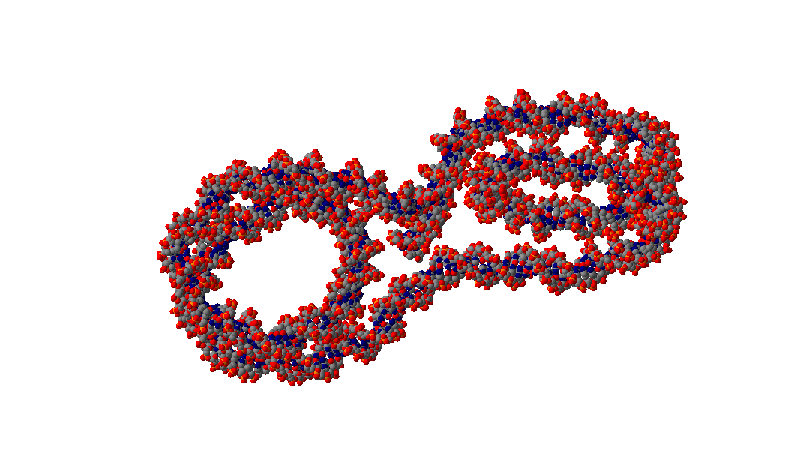
\includegraphics[width=.78\linewidth]{./Figures/bavdw.png}
  \caption{Baricentro VDW}
  \label{fig:sub33}
\end{subfigure}%
\begin{subfigure}{.5\textwidth}
  \centering
  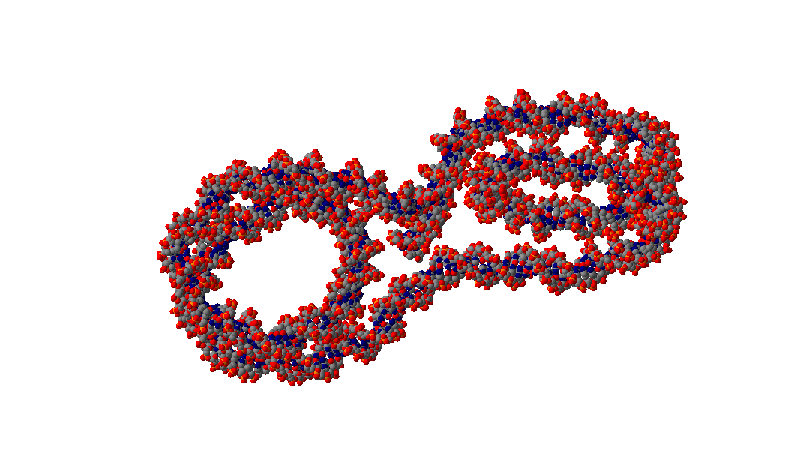
\includegraphics[width=.78\linewidth]{./Figures/bavdw.png}
  \caption{Centros de masa VDW}
  \label{fig:sub44}
\end{subfigure}
\begin{subfigure}{.5\textwidth}
  \centering
  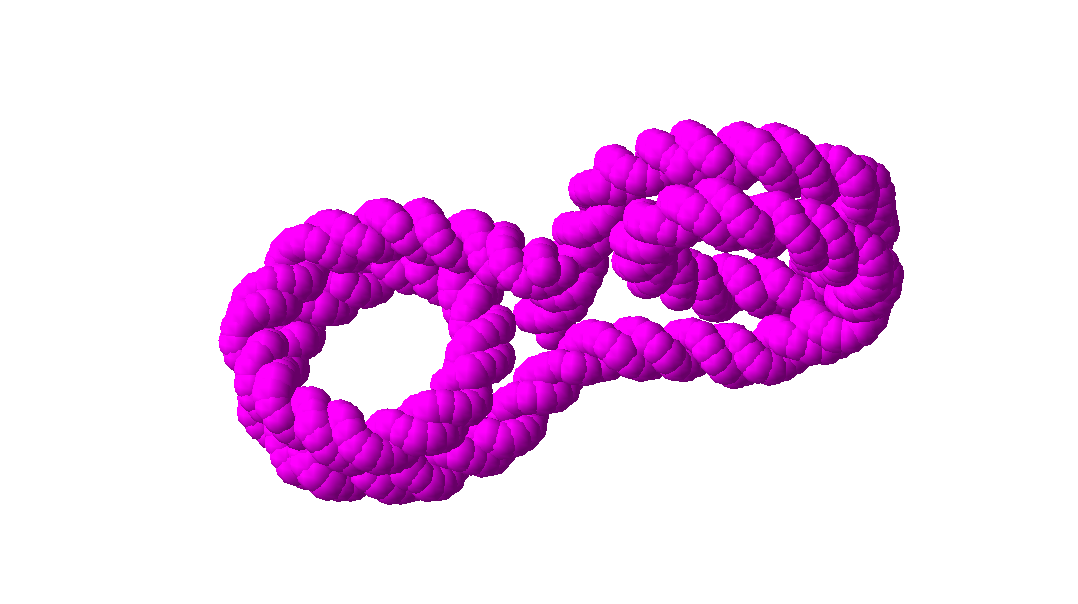
\includegraphics[width=.78\linewidth]{./Figures/a.png}
  \caption{Baricentro esferas ligadas}
  \label{fig:sub55}
\end{subfigure}%
\begin{subfigure}{.5\textwidth}
  \centering
  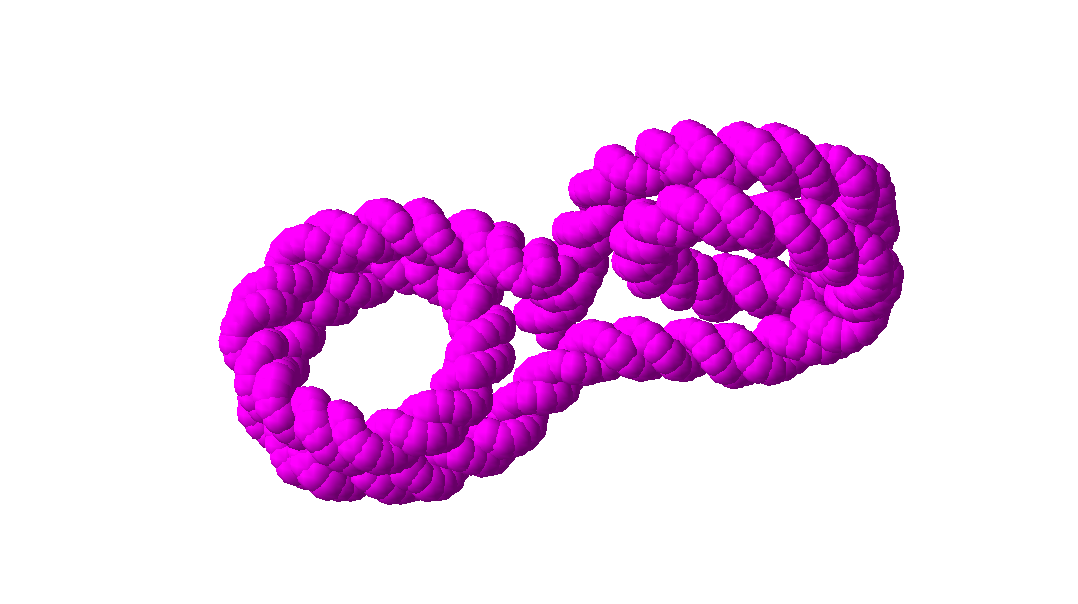
\includegraphics[width=.78\linewidth]{./Figures/a.png}
  \caption{Centros de masa esferas ligadas}
  \label{fig:sub66}
\end{subfigure}
\caption[Comparación de centros de masa y baricentros en Geant4 1ZBB]{Comparación representación centros de masa y baricentros en Geant4 para 1ZBB}
\label{h}
\end{figure}




\begin{figure}
\centering
\begin{subfigure}{.5\textwidth}
  \centering
  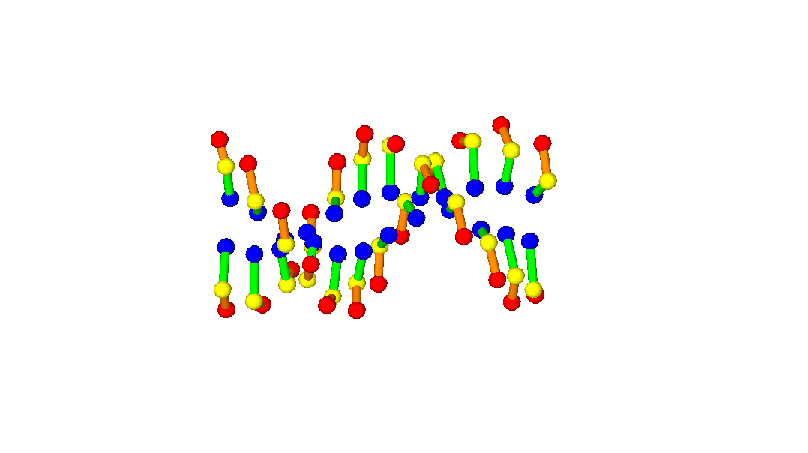
\includegraphics[width=.78\linewidth]{./Figures/1fzxresid.png}
  \caption{Baricentros residuos}
  \label{fig:sub111}
\end{subfigure}%
\begin{subfigure}{.5\textwidth}
  \centering
  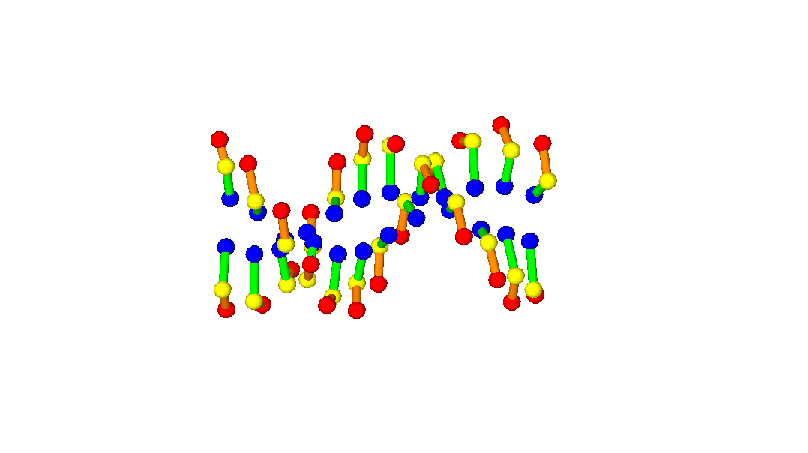
\includegraphics[width=.78\linewidth]{./Figures/1fzxresid.png}
  \caption{Centros de masa residuos}
  \label{fig:sub222}
\end{subfigure}
\begin{subfigure}{.5\textwidth}
  \centering
  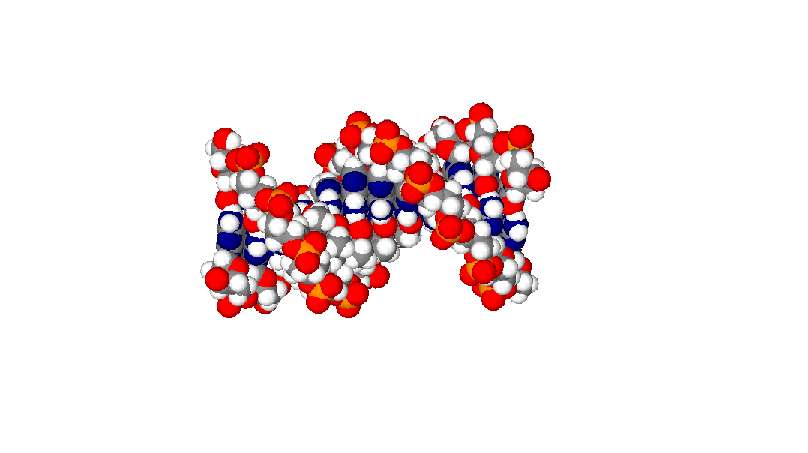
\includegraphics[width=.78\linewidth]{./Figures/1fzxvdw.png}
  \caption{Baricentro VDW}
  \label{fig:sub333}
\end{subfigure}%
\begin{subfigure}{.5\textwidth}
  \centering
  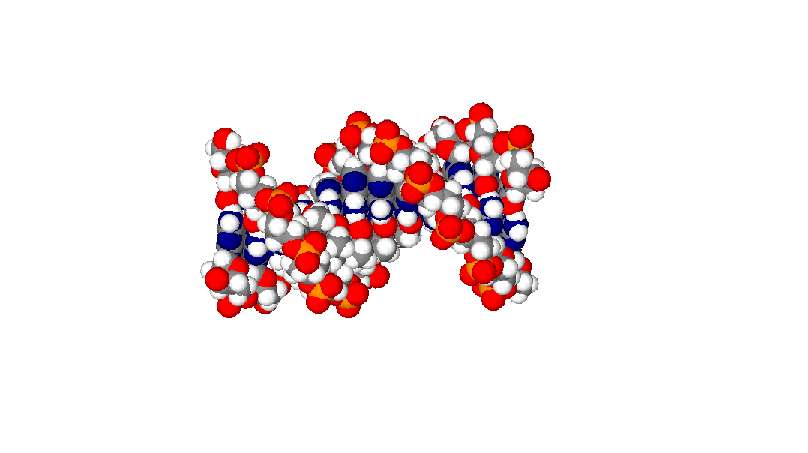
\includegraphics[width=.78\linewidth]{./Figures/1fzxvdw.png}
  \caption{Centros de masa VDW}
  \label{fig:sub444}
\end{subfigure}
\begin{subfigure}{.5\textwidth}
  \centering
  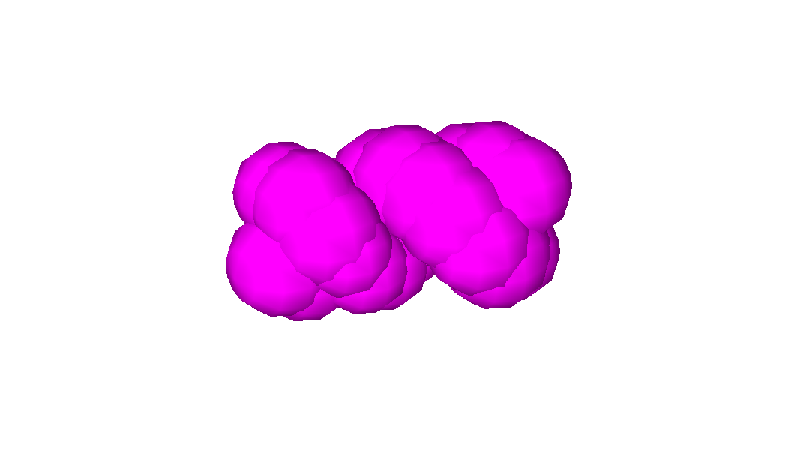
\includegraphics[width=.78\linewidth]{./Figures/1fzxba.png}
  \caption{Baricentro esferas ligadas}
  \label{fig:sub555}
\end{subfigure}%
\begin{subfigure}{.5\textwidth}
  \centering
  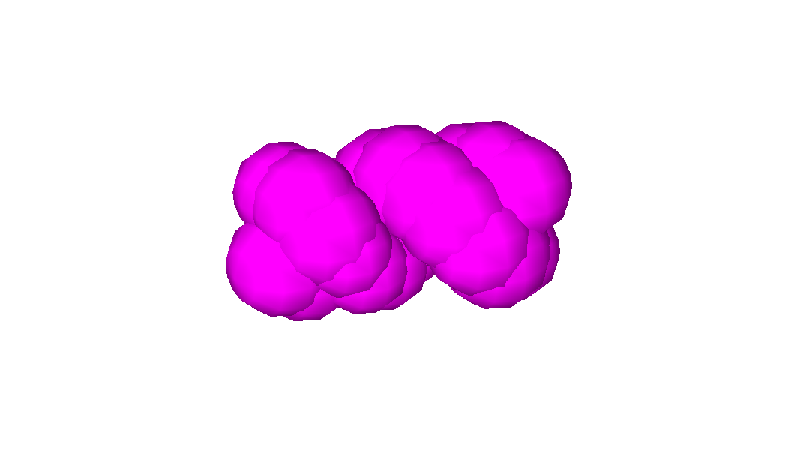
\includegraphics[width=.78\linewidth]{./Figures/1fzxba.png}
  \caption{Centros de masa esferas ligadas}
  \label{fig:sub666}
\end{subfigure}
\caption[Comparación de centros de masa y baricentros en Geant4 1FZX]{Comparación representación centros de masa y baricentros en Geant4 para 1FZX}
\label{hh}
\end{figure}




\begin{figure}[htbp]
    \centering
    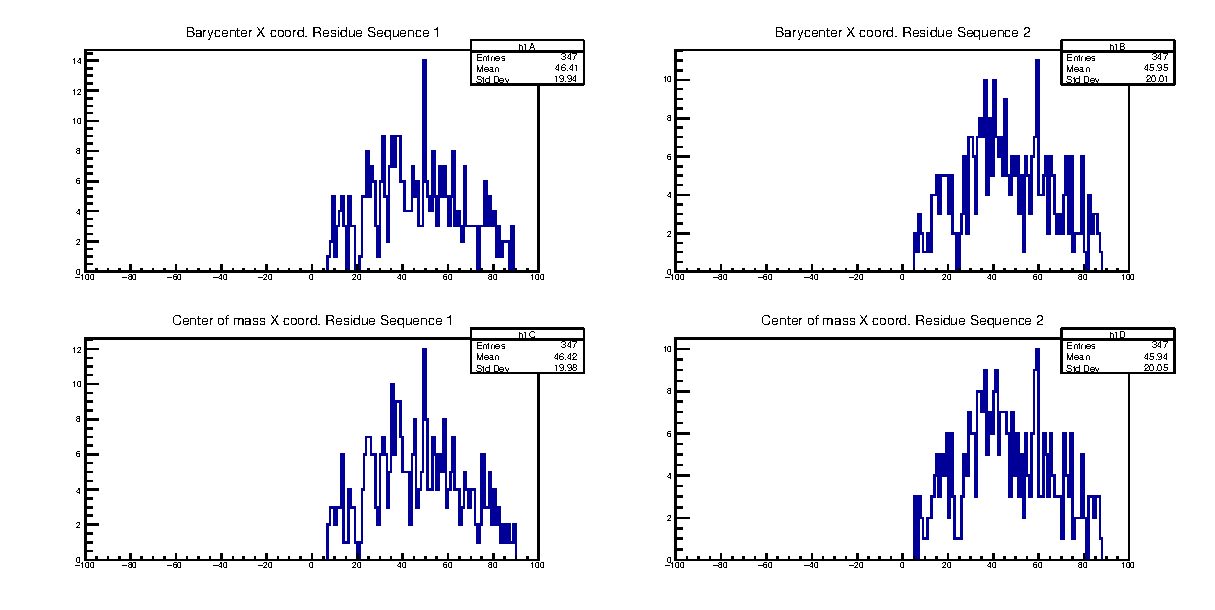
\includegraphics[width=1\linewidth]{./Figures/can1.eps}
  \caption[Baricentros en $x$ vs centros de masa en $x$ para 1ZBB]{Baricentros en $x$ vs centros de masa en $x$ para 1ZBB}
    \label{fig:canx}
\end{figure}

\begin{figure}[htbp]
    \centering
    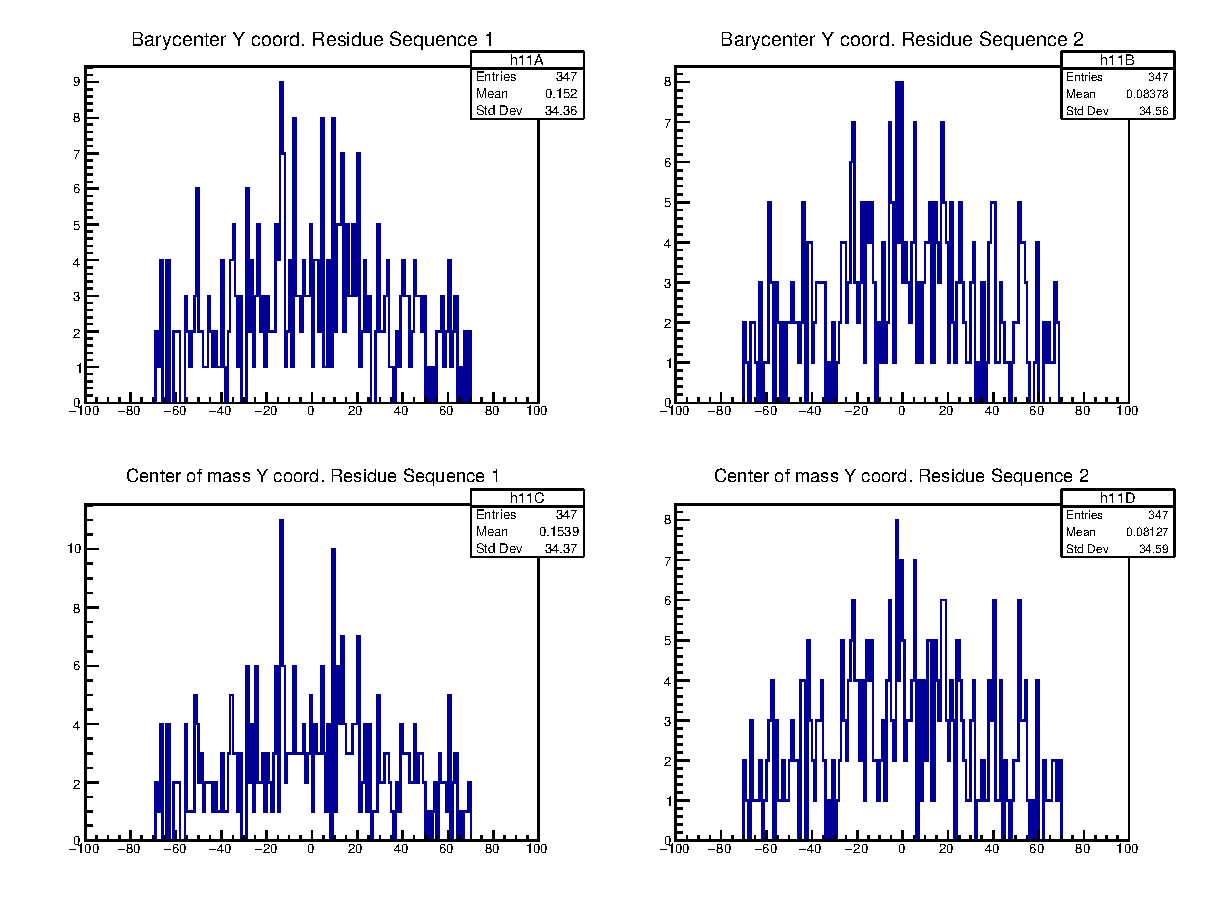
\includegraphics[width=1\linewidth]{./Figures/can2.eps}
    \caption[Baricentros en $y$ vs centros de masa en $y$ para 1ZBB]{Baricentros en $y$ vs centros de masa en $y$ para 1ZBB}
    \label{fig:cany}
\end{figure}

\begin{figure}[htbp]
    \centering
    \includegraphics[width=1\linewidth]{./Figures/can3.eps}
  \caption[Baricentros en $z$ vs centros de masa en $z$ para 1ZBB]{Baricentros en $z$ vs centros de masa en $z$ para 1ZBB}
    \label{fig:canz}
\end{figure}




\begin{figure}[htbp]
    \centering
    \includegraphics[width=1\linewidth]{./Figures/1fzx.eps}
  \caption[Baricentros en $x$ vs centros de masa en $x$ para 1FZX]{Baricentros en $x$ vs centros de masa en $x$ para 1FZX}
    \label{fig:cax}
\end{figure}

\begin{figure}[htbp]
    \centering
    \includegraphics[width=1\linewidth]{./Figures/1fzy.eps}
  \caption[Baricentros en $y$ vs centros de masa en $y$ para 1FZX]{Baricentros en $y$ vs centros de masa en $y$ para 1FZX}
    \label{fig:cay}
\end{figure}

\begin{figure}[htbp]
    \centering
    \includegraphics[width=1\linewidth]{./Figures/1fzz.eps}
  \caption[Baricentros en $z$ vs centros de masa en $z$ para 1FZX]{Baricentros en $z$ vs centros de masa en $z$ para 1FZX}
    \label{fig:caz}
\end{figure}



hablar algo de TER Y limitaciones
Hacer modificaciones de TER
mismas partículas?
centros de masa
PDB4DNA fue modificado de tal manera que en vez de hacer uso de las esferas ligadas a partir de baricentros usara centros de masa, para esto se uso el archivo PDBlib, primero se definió la masa de los diferentes elementos (véase anexo ~\ref{app:A}),y luego se usaron las clases bases ya definidas en PDBlib para hacer los respectivos cálculos de centros de masa(véase anexo ~\ref{app:B}).\\
